\documentclass[11pt,a4paper]{article}

% --- Essential Packages ---
\usepackage[utf8]{inputenc}
\usepackage[T1]{fontenc}
\usepackage{lmodern}
\usepackage[margin=1in,top=1.1in,bottom=1.1in]{geometry}
\usepackage{amsmath,amssymb,amsfonts,bm}
\usepackage{graphicx}
\usepackage{subcaption}
\usepackage{booktabs,tabularx,multirow,array}
\usepackage{xcolor}
\usepackage{tikz}
\usetikzlibrary{shapes.geometric, arrows.meta, positioning, calc, shadows, fit, backgrounds}
\usepackage{fancyhdr}
\usepackage{titlesec}
\usepackage{microtype}
\usepackage{enumitem}
\usepackage{placeins}
\usepackage{float}
\renewcommand{\topfraction}{0.88}
\renewcommand{\bottomfraction}{0.80}
\renewcommand{\textfraction}{0.08}
\renewcommand{\floatpagefraction}{0.85}
\usepackage[colorlinks=true,linkcolor=navyblue,citecolor=tealblue,urlcolor=navyblue]{hyperref}

% --- Color Palette ---
\definecolor{navyblue}{RGB}{20, 45, 110}
\definecolor{tealblue}{RGB}{13, 148, 136}
\definecolor{darkslate}{RGB}{30, 41, 59}
\definecolor{softgray}{RGB}{248, 250, 252}
\definecolor{bordergray}{RGB}{226, 232, 240}
\definecolor{accentpurple}{RGB}{124, 58, 237}
\definecolor{accentorange}{RGB}{234, 88, 12}
\definecolor{accentgreen}{RGB}{22, 163, 74}

% --- Page Header & Footer ---
\pagestyle{fancy}
\fancyhf{}
\fancyhead[L]{\small\sffamily\color{gray} MagMat-Discovery $\cdot$ Technical Report}
\fancyhead[R]{\small\sffamily\color{gray} Sachin Poudel}
\fancyfoot[C]{\small\sffamily\color{darkslate}\thepage}
\renewcommand{\headrulewidth}{0.4pt}
\renewcommand{\footrulewidth}{0.0pt}

% --- Section Heading Styling ---
\titleformat{\section}
  {\Large\sffamily\bfseries\color{navyblue}}
  {\thesection}{1em}{}[\titlerule]
\titleformat{\subsection}
  {\large\sffamily\bfseries\color{darkslate}}
  {\thesubsection}{0.8em}{}
\titleformat{\subsubsection}
  {\normalsize\sffamily\bfseries\color{tealblue}}
  {\thesubsubsection}{0.6em}{}

% --- Spacing Adjustments ---
\setlist{itemsep=2pt, topsep=3pt}

\begin{document}

% ==============================================================================
% COVER PAGE
% ==============================================================================
\hypersetup{pageanchor=false}
\begin{titlepage}
    \centering
    \vspace*{1.5cm}
    
    {\Huge\sffamily\bfseries\color{navyblue} MagMat-Discovery}\\[0.4cm]
    {\LARGE\sffamily\color{darkslate} Physics-Informed Machine Learning and Screening for Magnetic Materials}\\[0.8cm]
    
    
\begin{tikzpicture}
        \draw[tealblue, line width=2.5pt] (0,0) -- (12,0);
        \draw[navyblue, line width=1.0pt] (0,-0.15) -- (12,-0.15);
    \end{tikzpicture}\\[1.2cm]
    
    {\Large\sffamily\bfseries System Architecture, Methodology \& Model Validation}\\[0.5cm]
    {\large\sffamily Technical Report \& Model Guide}\\[3.0cm]
    
    \begin{minipage}{0.75\textwidth}
        \centering
        \sffamily
        \begin{tabular}{r l}
            \textbf{\color{navyblue} Author:} & \Large\textbf{Sachin Poudel} \\[0.3cm]
            \textbf{\color{navyblue} Project:} & MagMat-Discovery Platform \\[3pt]
            \textbf{\color{navyblue} Web Platform:} & Interactive Streamlit Discovery Engine \\[3pt]
            \textbf{\color{navyblue} Date:} & September 2026 \\
        \end{tabular}
    \end{minipage}
    
    \vfill
\end{titlepage}
\hypersetup{pageanchor=true}

% ==============================================================================
% TABLE OF CONTENTS
% ==============================================================================
\newpage
\pagenumbering{roman}
\tableofcontents
\newpage
\pagenumbering{arabic}

% ==============================================================================
% EXECUTIVE SUMMARY / ABSTRACT
% ==============================================================================
\section*{Executive Summary}
\addcontentsline{toc}{section}{Executive Summary}

Discovering permanent magnets with reduced rare-earth content is important for electric vehicles, wind turbines, and industrial machinery. Useful candidates must meet three criteria: Curie temperature $T_C > 400\,\text{K}$, saturation magnetization $\mu_0 M_s > 1.0\,\text{T}$, and coercivity $H_c > 800\,\text{kA/m}$. However, machine learning for magnetic materials is challenging because intrinsic properties depend on atomic chemistry while extrinsic properties depend on grain microstructure. Furthermore, random data splits cause leakage between identical compositions, and unconstrained models can make unphysical predictions.

\textbf{MagMat-Discovery} addresses these challenges through four objectives:
\begin{enumerate}[leftmargin=1.5em]
    \item \textbf{Multi-Target Modeling:} Predict 8 intrinsic and extrinsic magnetic properties covering phase, transition temperatures, and hysteresis behavior.
    \item \textbf{Grouped Evaluation:} Evaluate models with 5-fold grouped cross-validation by chemical formula to prevent data leakage.
    \item \textbf{Physics Cascades:} Connect intrinsic predictions ($K_1, M_s$) to extrinsic properties ($H_c$ and $(BH)_{\max}$) using micromagnetic equations and physical bounds.
    \item \textbf{Calibrated Uncertainty:} Provide 90\% conformal intervals for every continuous property alongside an interactive screening app.
\end{enumerate}

By combining experimental data, physical features, the \textbf{MagFormer} graph model, ensembles, and conformal calibration, the platform accurately predicts magnetic properties and provides physically bounded rankings for magnet discovery.

\vspace{0.4cm}
\noindent\textbf{Keywords:} Magnetic Materials, Physics-Informed Machine Learning, Graph Transformers, Conformal Calibration, Coercivity, Permanent Magnets, Materials Screening.

\clearpage
% ==============================================================================
% GLOSSARY OF TERMS
% ==============================================================================
\section*{Glossary of Key Terms}
\addcontentsline{toc}{section}{Glossary of Key Terms}

Table~\ref{tab:glossary} summarizes the primary magnetic properties and machine learning terminology used throughout this report.

\begin{table}[H]
\centering
\small\sffamily
\caption{Glossary of magnetic properties, physical units, and computational terms.}
\label{tab:glossary}
\begin{tabularx}{\textwidth}{l c X}
\toprule
\textbf{\color{navyblue}Term} & \textbf{\color{navyblue}Unit} & \textbf{\color{navyblue}Definition} \\
\midrule
$T_C$ (Curie Temp.) & $\text{K}$ & Temperature above which a ferromagnet loses spontaneous magnetization. \\
$T_N$ (Néel Temp.) & $\text{K}$ & Temperature above which an antiferromagnet becomes paramagnetic. \\
$M_s$ (Saturation Mag.) & $\text{emu/g}$ or $\text{T}$ & Maximum magnetization in an applied field, reported in $\text{emu/g}$ or $\mu_0 M_s$ ($\text{T}$). \\
$H_c$ (Coercivity) & $\text{A/m}$ or $\text{kA/m}$ & Magnetic field required to reduce magnetization to zero after saturation. \\
$K_1$ (Anisotropy Constant) & $\text{J/m}^3$ & Energy density required to rotate magnetization away from the preferred crystal axis. \\
$(BH)_{\max}$ (Energy Product) & $\text{kJ/m}^3$ & Maximum stored magnetic energy density; main figure of merit for permanent magnets. \\
$\theta_p$ (Paramagnetic Curie Temp.) & $\text{K}$ & High-temperature intercept from Curie-Weiss susceptibility fitting. \\
FM / AFM / NM & Discrete & Ferromagnetic, Antiferromagnetic, or Non-magnetic ground-state ordering. \\
\midrule
Out-of-Fold (OOF) & -- & Predictions on held-out validation data, avoiding data leakage. \\
Conformal Range & Physical & Uncertainty window covering the true value 90\% of the time. \\
dex & $\log_{10}$ & Decimal order of magnitude. An error of 0.65 dex means a factor of $10^{0.65} \approx 4.5$. \\
\bottomrule
\end{tabularx}
\end{table}

\clearpage

% ==============================================================================
% 1. DATA AND PARTITIONING
% ==============================================================================
\section{Data and Partitioning}

\subsection{Data Sources}
\label{sec:data_sources}
The platform uses three primary data sources:
\begin{itemize}[leftmargin=1.5em]
    \item \textbf{NEMAD Database:} 51,394 experimental records \cite{nemad2025} across all 8 target properties.
    \item \textbf{Materials Project:} Crystal symmetries (space groups 1--230, crystal systems, and densities) \cite{materials_project}. DFT energies and moments are excluded to prevent target leakage.
    \item \textbf{Bilbao MAGNDATA:} Magnetic space groups and Shubnikov symmetry classifications.
\end{itemize}

\subsection{Data Cleaning and Grouped Splits}
\label{sec:data_splits}
Chemical formulas are simplified to lowest integer ratios with \texttt{pymatgen} (e.g., $\text{Fe}_6\text{Pt}_2 \to \text{Fe}_3\text{Pt}$). Properties spanning multiple orders of magnitude ($H_c, K_1, (BH)_{\max}$) are log-transformed.

To evaluate generalization to unseen materials, models are tested with 5-fold cross-validation grouped by chemical formula (\texttt{GroupKFold}). All entries with the same formula or crystal phase stay in the same split, ensuring test folds contain only new compounds.

% ==============================================================================
% 2. METHODOLOGY
% ==============================================================================
\clearpage
\section{Methodology}

\subsection{Architecture and Provenance}
\label{sec:provenance}

Figure~\ref{fig:methodology_flowchart} shows the overall workflow of MagMat-Discovery, distinguishing external resources from in-house algorithms (Table~\ref{tab:provenance}). External databases and foundation models provide experimental records, crystal symmetries, and 3D crystal generation. All regressors, phase classifiers, micromagnetic cascades, and uncertainty calibrators were trained and evaluated in-house.

\begin{figure}[!t]
\centering
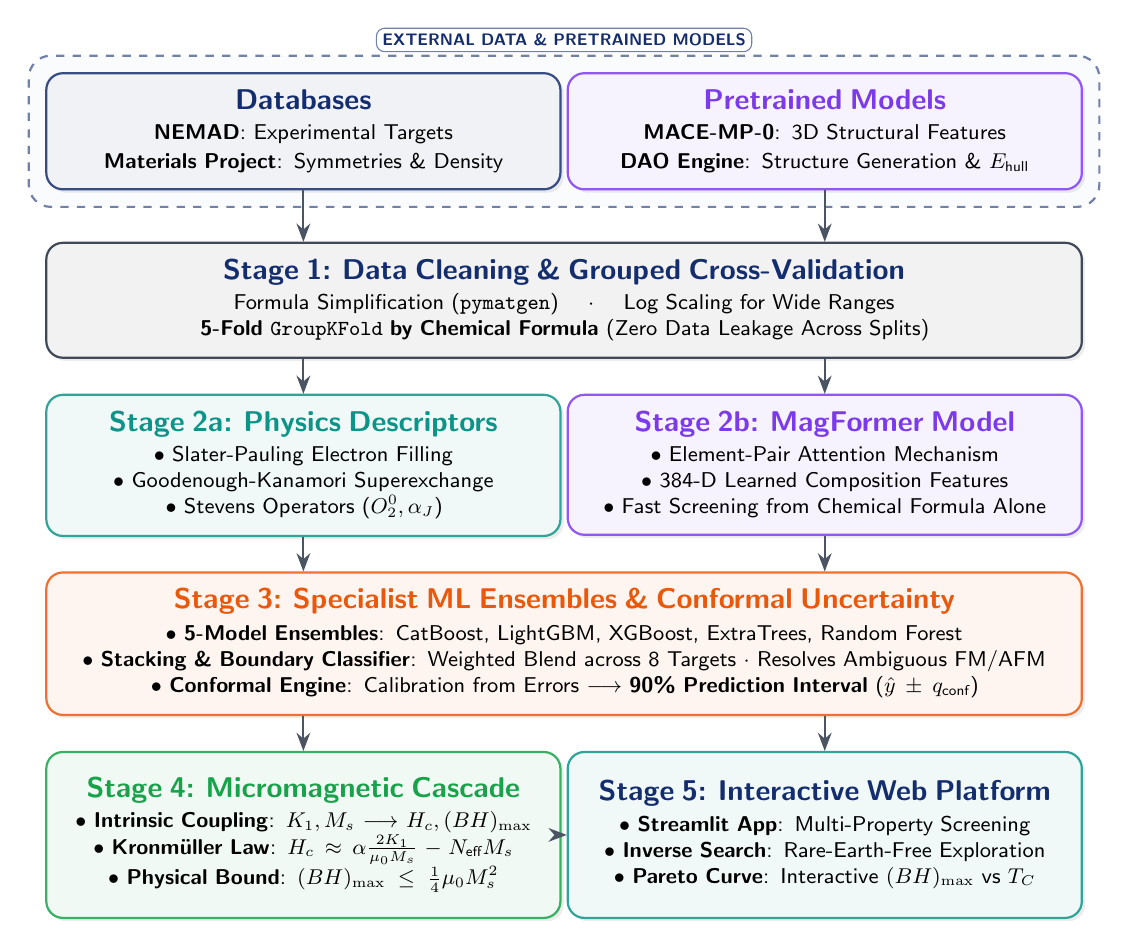
\begin{tikzpicture}[
    scale=0.86, every node/.style={transform shape},
    >=Stealth,
    card/.style={
        rectangle, rounded corners=6pt,
        draw=#1!85, fill=#1!6,
        thick, inner sep=7pt, align=center,
        font=\small\sffamily,
        drop shadow={shadow xshift=1.2pt, shadow yshift=-1.2pt, opacity=0.15}
    },
    groupbox/.style={
        rectangle, rounded corners=8pt,
        draw=#1!60, fill=#1!2,
        dashed, line width=0.8pt,
        inner sep=6pt
    },
    grouplabel/.style={
        font=\scriptsize\sffamily\bfseries\color{#1},
        fill=white, rounded corners=3pt, draw=#1!60, thin, inner sep=2.5pt
    },
    arrow/.style={->, thick, draw=darkslate!80, rounded corners=3pt},
    darrow/.style={->, thick, dashed, draw=#1!80, rounded corners=3pt}
]

% ==============================================================================
% LEVEL 1: EXTERNAL DATABASES & PRETRAINED MODELS (2 CARDS)
% ==============================================================================
\node[card=navyblue, text width=7.1cm, minimum height=1.45cm] (dbs) at (-3.85, 0) {
    \textbf{\large\color{navyblue} Databases}\\[0.06cm]
    \textbf{NEMAD}: Experimental Targets\\[1pt]
    \textbf{Materials Project}: Symmetries \& Density
};

\node[card=accentpurple, text width=7.1cm, minimum height=1.45cm] (foundations) at (3.85, 0) {
    \textbf{\large\color{accentpurple} Pretrained Models}\\[0.06cm]
    \textbf{MACE-MP-0}: 3D Structural Features\\[1pt]
    \textbf{DAO Engine}: Structure Generation \& $E_{\text{hull}}$
};

\begin{scope}[on background layer]
    \node[groupbox=navyblue, fit=(dbs) (foundations)] (box1) {};
    \node[grouplabel=navyblue, above=1pt of box1.north] {EXTERNAL DATA \& PRETRAINED MODELS};
\end{scope}

% ==============================================================================
% LEVEL 2: DATA CLEANING & GROUP SPLITS (1 WIDE CARD)
% ==============================================================================
\node[card=darkslate, text width=14.8cm, below=0.50cm of box1] (prep) {
    \textbf{\large\color{navyblue} Stage 1: Data Cleaning \& Grouped Cross-Validation}\\[0.06cm]
    Formula Simplification (\texttt{pymatgen}) \quad $\cdot$ \quad Log Scaling for Wide Ranges\\
    \textbf{5-Fold \texttt{GroupKFold} by Chemical Formula} (Zero Data Leakage Across Splits)
};

\draw[arrow] (dbs.south) -- (prep.north -| dbs.center);
\draw[arrow] (foundations.south) -- (prep.north -| foundations.center);

% ==============================================================================
% LEVEL 3: DUAL REPRESENTATION LAYER (2 CARDS)
% ==============================================================================
\node[card=tealblue, text width=7.1cm, minimum height=1.75cm, below=0.52cm of prep.south -| dbs.center] (physics) {
    \textbf{\large\color{tealblue} Stage 2a: Physics Descriptors}\\[0.06cm]
    $\bullet$ Slater-Pauling Electron Filling\\
    $\bullet$ Goodenough-Kanamori Superexchange\\
    $\bullet$ Stevens Operators ($O_2^0, \alpha_J$)
};

\node[card=accentpurple, text width=7.1cm, minimum height=1.75cm, below=0.52cm of prep.south -| foundations.center] (magformer) {
    \textbf{\large\color{accentpurple} Stage 2b: MagFormer Model}\\[0.06cm]
    $\bullet$ Element-Pair Attention Mechanism\\
    $\bullet$ 384-D Learned Composition Features\\
    $\bullet$ Fast Screening from Chemical Formula Alone
};

\draw[arrow] (prep.south -| physics.center) -- (physics.north);
\draw[arrow] (prep.south -| magformer.center) -- (magformer.north);

% ==============================================================================
% LEVEL 4: MACHINE LEARNING & CONFORMAL UNCERTAINTY (1 WIDE CARD)
% ==============================================================================
\node[card=accentorange, text width=14.8cm, below=0.52cm of $(physics.south)!0.5!(magformer.south)$] (ml) {
    \textbf{\large\color{accentorange} Stage 3: Specialist ML Ensembles \& Conformal Uncertainty}\\[0.08cm]
    $\bullet$ \textbf{5-Model Ensembles}: CatBoost, LightGBM, XGBoost, ExtraTrees, Random Forest\\
    $\bullet$ \textbf{Stacking \& Boundary Classifier}: Weighted Blend across 8 Targets $\cdot$ Resolves Ambiguous FM/AFM\\
    $\bullet$ \textbf{Conformal Engine}: Calibration from Errors $\longrightarrow$ \textbf{90\% Prediction Interval} ($\hat{y} \pm q_{\text{conf}}$)
};

\draw[arrow] (physics.south) -- (ml.north -| physics.center);
\draw[arrow] (magformer.south) -- (ml.north -| magformer.center);

% ==============================================================================
% LEVEL 5: PHYSICAL CASCADE & WEB DISCOVERY (2 CARDS)
% ==============================================================================
\node[card=accentgreen, text width=7.1cm, minimum height=2.45cm, below=0.52cm of ml.south -| dbs.center] (cascade) {
    \textbf{\large\color{accentgreen} Stage 4: Micromagnetic Cascade}\\[0.06cm]
    $\bullet$ \textbf{Intrinsic Coupling}: $K_1, M_s \longrightarrow H_c, (BH)_{\max}$\\
    $\bullet$ \textbf{Kronmüller Law}: $H_c \approx \alpha \frac{2 K_1}{\mu_0 M_s} - N_{\text{eff}} M_s$\\
    $\bullet$ \textbf{Physical Bound}: $(BH)_{\max} \le \frac{1}{4} \mu_0 M_s^2$
};

\node[card=tealblue, text width=7.1cm, minimum height=2.45cm, below=0.52cm of ml.south -| foundations.center] (app) {
    \textbf{\large\color{navyblue} Stage 5: Interactive Web Platform}\\[0.06cm]
    $\bullet$ \textbf{Streamlit App}: Multi-Property Screening\\
    $\bullet$ \textbf{Inverse Search}: Rare-Earth-Free Exploration\\
    $\bullet$ \textbf{Pareto Curve}: Interactive $(BH)_{\max}$ vs $T_C$
};

\draw[arrow] (ml.south -| cascade.center) -- (cascade.north);
\draw[arrow] (ml.south -| app.center) -- (app.north);
\draw[arrow] (cascade.center -| cascade.east) -- (cascade.center -| app.west);

\end{tikzpicture}
\caption{Workflow of MagMat-Discovery, showing external resources, in-house representations, 5-model ensembles, physical cascades, and candidate screening.}
\label{fig:methodology_flowchart}
\end{figure}

Table~\ref{tab:provenance} lists the data sources, pretrained models, and in-house components used in the pipeline.

\begin{table}[!t]
\centering
\small\sffamily
\caption{Data sources, models, and algorithmic components in MagMat-Discovery.}
\label{tab:provenance}
\begin{tabularx}{\textwidth}{>{\bfseries}p{4.0cm} p{2.2cm} p{3.6cm} >{\raggedright\arraybackslash}X}
\toprule
\textbf{\color{navyblue}Component} & \textbf{\color{navyblue}Type} & \textbf{\color{navyblue}Source} & \textbf{\color{navyblue}Role in Pipeline} \\
\midrule
Materials Project \cite{materials_project} & External DB & Open DFT repository & Crystal symmetries and densities (energies/moments excluded). \\
NEMAD Database \cite{nemad2025} & External DB & Experimental literature & Target measurements for all 8 magnetic properties. \\
MACE-MP-0 \cite{mace2022} & Pretrained & Equivariant GNN & 3D structural features for compounds with known coordinates. \\
DAO Engine \cite{dao2026} & Pretrained & Diffusion model & Generates 3D unit cells (DAO-G) and checks stability $E_{\text{hull}}$ (DAO-P). \\
\midrule
MagFormer & In-House & Trained in this work & Maps chemical formulas to 384-D features without 3D coordinates. \\
Physics Descriptors & In-House & Domain physics & Electron counts (VEC), superexchange proxies, Stevens factors. \\
5-Model Ensembles & In-House & 5-fold grouped training & Blends CatBoost, LightGBM, XGBoost, ExtraTrees, Random Forest. \\
Boundary Classifier & In-House & Ambiguous data & Resolves ambiguous FM vs. AFM phase predictions. \\
Micromagnetic Cascade & In-House & Micromagnetic theory \cite{kronmuller2003} & Enforces Kronmüller coercivity and $(BH)_{\max} \le \frac{1}{4}\mu_0 M_s^2$. \\
Conformal Engine & In-House & Validation residuals \cite{vovk2005} & Provides 90\% prediction intervals for continuous properties. \\
\bottomrule
\end{tabularx}
\end{table}

\subsection{Representations and Structure Synthesis}
\label{sec:physics_descriptors}
\label{sec:magformer_architecture}
\label{sec:dao_screening}

The pipeline represents materials using three complementary methods:

\textbf{1. Physics Descriptors:} Features organized into four tiers (Appendix~\ref{sec:appendix_physics}):
\begin{itemize}[leftmargin=1.5em]
    \item \emph{Tier 1 (Composition):} Mass fractions, atomic numbers, covalent radii, and electronegativities.
    \item \emph{Tier 2 (Electronic Structure):} Valence electron count relative to the Slater-Pauling peak ($\text{VEC} \approx 8.3$), exchange rules, and spin-orbit coupling ($\propto Z^4$).
    \item \emph{Tier 3 (Crystal Field):} Crystal family indicators and Stevens factors ($O_2^0, \alpha_J$) for easy-axis preference.
    \item \emph{Tier 4 (3D Features):} Atomic representations from MACE-MP-0 \cite{mace2022} when 3D coordinates exist.
\end{itemize}

\textbf{2. MagFormer Model:} For screening materials without crystal coordinates, \textbf{MagFormer} maps chemical formulas to 384-dimensional feature vectors using self-attention (Appendix~\ref{sec:appendix_magformer}).

\textbf{3. DAO Structure Generation:} When 3D coordinates are needed, the pretrained DAO model \cite{dao2026} generates unit cells (DAO-G) and calculates stability ($E_{\text{hull}}$ via DAO-P). Materials with $E_{\text{hull}} < 0.05\,\text{eV/atom}$ are considered synthesizable.

\subsection{Ensembles, Cascades, and Uncertainty}
\label{sec:ensembles_and_cascades}

We predict each property using an ensemble of five machine learning models: CatBoost, LightGBM, XGBoost, ExtraTrees, and Random Forest. Their predictions are combined through weighted averaging (non-negative least squares). For magnetic phase, a secondary classifier resolves borderline cases where ferromagnetic and antiferromagnetic probabilities are close ($|P(\text{FM}) - P(\text{AFM})| < 0.20$).

To prevent predictions that violate the laws of physics, the pipeline uses a step-by-step physical cascade:
\begin{enumerate}[leftmargin=1.5em]
    \item Intrinsic properties ($K_1$ and $M_s$) are predicted first.
    \item These predictions feed into the coercivity ($H_c$) and energy product ($(BH)_{\max}$) models, ensuring coercivity follows the Kronmüller relationship \cite{kronmuller2003}:
    \begin{equation}
        H_c \approx \alpha_{\text{micro}} \frac{2 K_1}{\mu_0 M_s} - N_{\text{eff}} M_s
        \label{eq:kronmuller}
    \end{equation}
    where $\alpha_{\text{micro}}$ accounts for grain defects and $N_{\text{eff}}$ is the demagnetizing factor.
    \item Predicted energy products are capped at the theoretical limit: $(BH)_{\max} \le \frac{1}{4}\mu_0 M_s^2$.
\end{enumerate}

Every continuous prediction includes a calibrated uncertainty range using conformal prediction \cite{vovk2005}. By taking the 90th percentile of absolute errors on held-out validation data:
\begin{equation}
    q_{\text{conf}} = \text{Quantile}_{0.90} \left( \{ |y_i - \hat{y}_i| \}_{i=1}^n \right)
\end{equation}
we provide an error window $[\hat{y} - q_{\text{conf}},\, \hat{y} + q_{\text{conf}}]$ that covers the true value 90\% of the time.

% ==============================================================================
% 3. MODEL VALIDATION
% ==============================================================================
\clearpage
\section{Model Validation}

\subsection{Benchmark Performance}
\label{sec:master_benchmark}

Models are evaluated using 5-fold cross-validation grouped by chemical formula (Section~\ref{sec:data_splits}). Performance is measured by the coefficient of determination ($R^2$) and mean absolute error (MAE). MAE is reported in physical units ($\text{K}, \text{emu/g}$) or decimal orders of magnitude ($\log_{10}$ error) for wide-range properties ($H_c, K_1, (BH)_{\max}$). Table~\ref{tab:master_metrics} reports benchmark results across all 8 targets.

\begin{table}[!t]
\centering
\small\sffamily
\caption{Comprehensive 5-fold GroupKFold cross-validation results across all 8 magnetic targets.}
\label{tab:master_metrics}
\resizebox{\textwidth}{!}{%
\begin{tabular}{c l c c r r r l}
\toprule
\textbf{\color{navyblue}\#} & \textbf{\color{navyblue}Target Property} & \textbf{\color{navyblue}Unit} & \textbf{\color{navyblue}Scale} & \textbf{\color{navyblue}Count $n$} & \textbf{\color{navyblue}Primary Metric} & \textbf{\color{navyblue}Mean Error} & \textbf{\color{navyblue}Practical Use} \\
\midrule
1 & Ground-State Phase & Discrete & Class & 35,045 & \textbf{91.9\% Accuracy} & Macro $F_1$: 0.908 & \textbf{Strong} (Reliable phase filtering) \\
2 & Curie Temperature ($T_C$) & $\text{K}$ & Linear & 15,518 & \textbf{$R^2 = 0.816$} & $\text{MAE} = 69.8\,\text{K}$ & \textbf{Strong} (Thermal threshold filter) \\
3 & Néel Temperature ($T_N$) & $\text{K}$ & Linear & 7,734 & \textbf{$R^2 = 0.741$} & $\text{MAE} = 48.6\,\text{K}$ & \textbf{Strong} (Accurate AFM boundary) \\
4 & Anisotropy Constant ($K_1$) & $\text{J/m}^3$ & Symlog & 3,938 & \textbf{$R^2 = 0.461$} & $\text{MAE} = 0.95\,\text{dex}$ & \textbf{Moderate} (Easy-axis candidate ranking) \\
5 & Coercivity ($H_c$) & $\text{A/m}$ & $\log_{10}$ & 6,980 & \textbf{$R^2 = 0.622$} & $\text{MAE} = 0.65\,\text{dex}$ & \textbf{Moderate} (Hard vs soft screening) \\
6 & Saturation Magnetization ($M_s$) & $\text{emu/g}$ & Linear & 7,619 & \textbf{$R^2 = 0.539$} & $\text{MAE} = 26.1\,\text{emu/g}$ & \textbf{Moderate} (Moment estimation) \\
7 & Energy Product ($(BH)_{\max}$) & $\text{kJ/m}^3$ & $\log_{10}$ & 1,379 & \textbf{$R^2 = 0.507$} & $\text{MAE} = 0.27\,\text{dex}$ & \textbf{Moderate} (Bounded density estimate) \\
8 & Paramagnetic Curie Temp. ($\theta_p$) & $\text{K}$ & Linear & 5,474 & \textbf{$R^2 = 0.607$} & $\text{MAE} = 64.7\,\text{K}$ & \textbf{Moderate} (Exchange coupling sign) \\
\bottomrule
\end{tabular}%
}
\end{table}

\subsection{Parity Analysis}
\label{sec:parity_analysis}

Performance reflects the difference between intrinsic properties (set by chemistry) and extrinsic properties (set by microstructure):

\textbf{Transition Temperatures ($T_C$ and $T_N$):} Curie and Néel temperatures achieve high accuracy ($R^2 = 0.82$ and $0.74$, Figure~\ref{fig:pair_temperatures}) because ordering temperatures depend directly on chemical bonding and composition.

\begin{figure}[!t]
    \centering
    \begin{subfigure}[b]{0.485\textwidth}
        \centering
        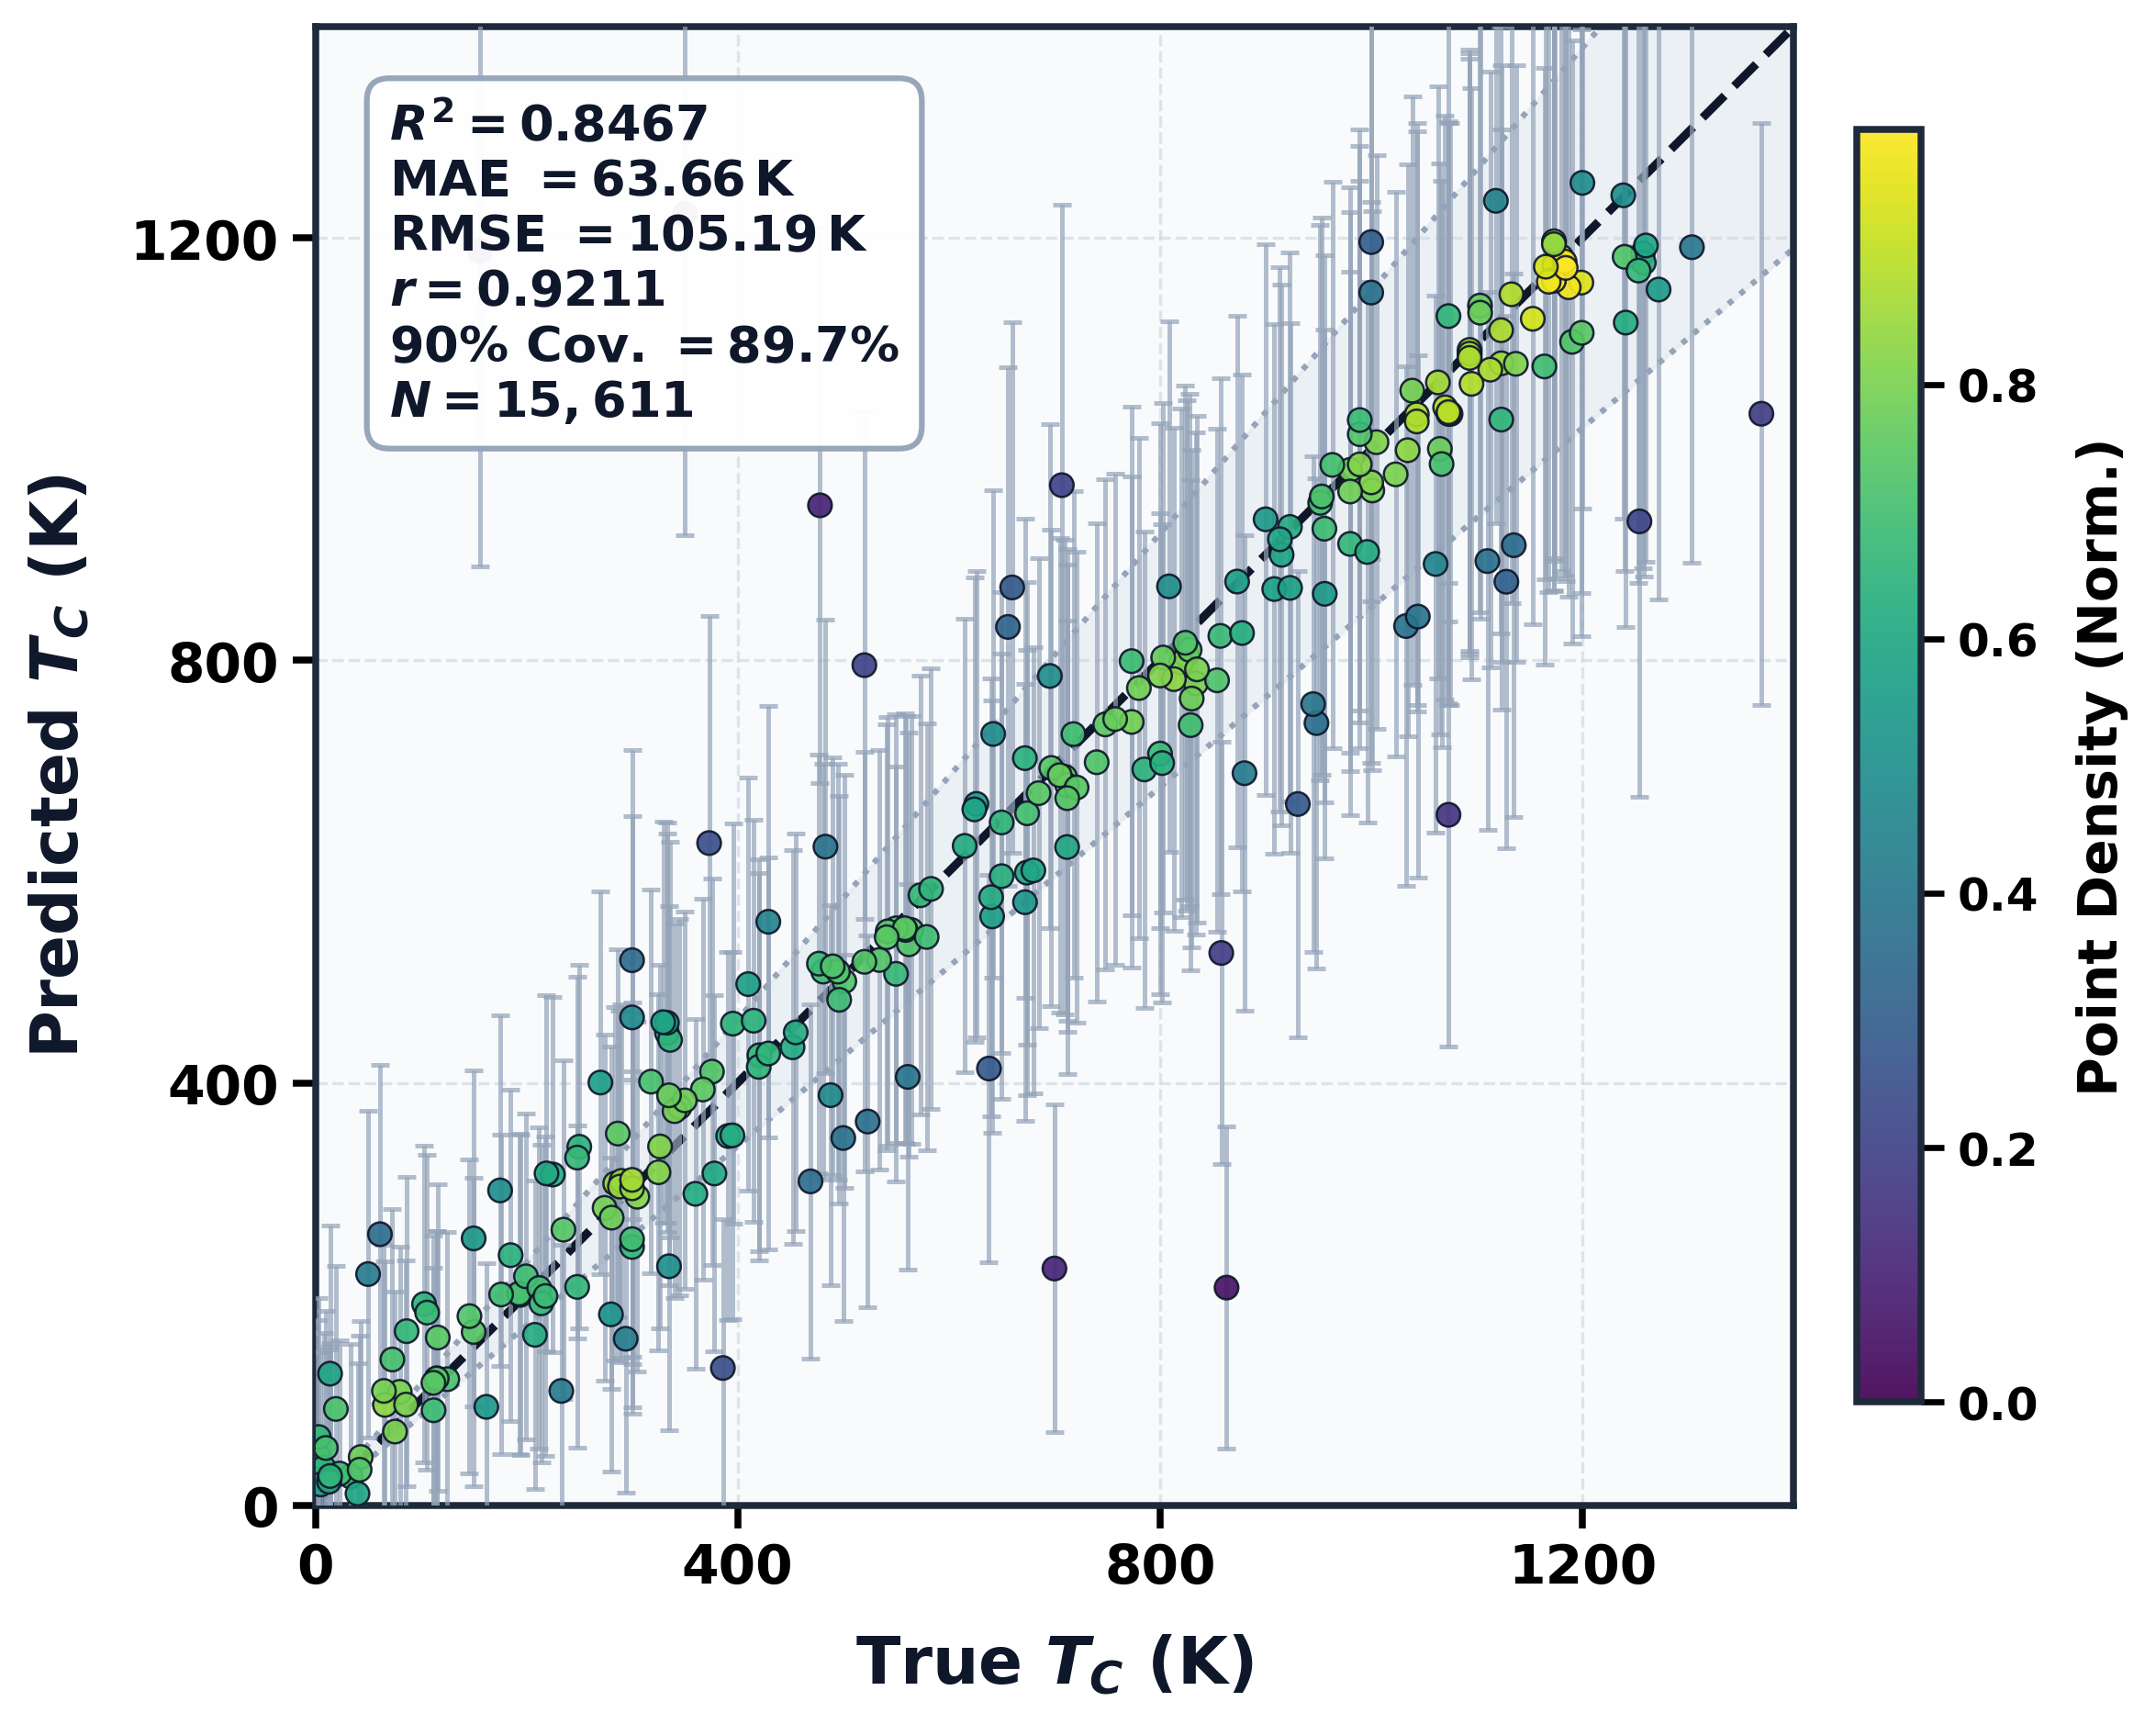
\includegraphics[width=\textwidth]{figures/curie_parity.png}
        \caption{Curie Temperature ($T_C$) Parity}
        \label{fig:curie_parity}
    \end{subfigure}
    \hfill
    \begin{subfigure}[b]{0.485\textwidth}
        \centering
        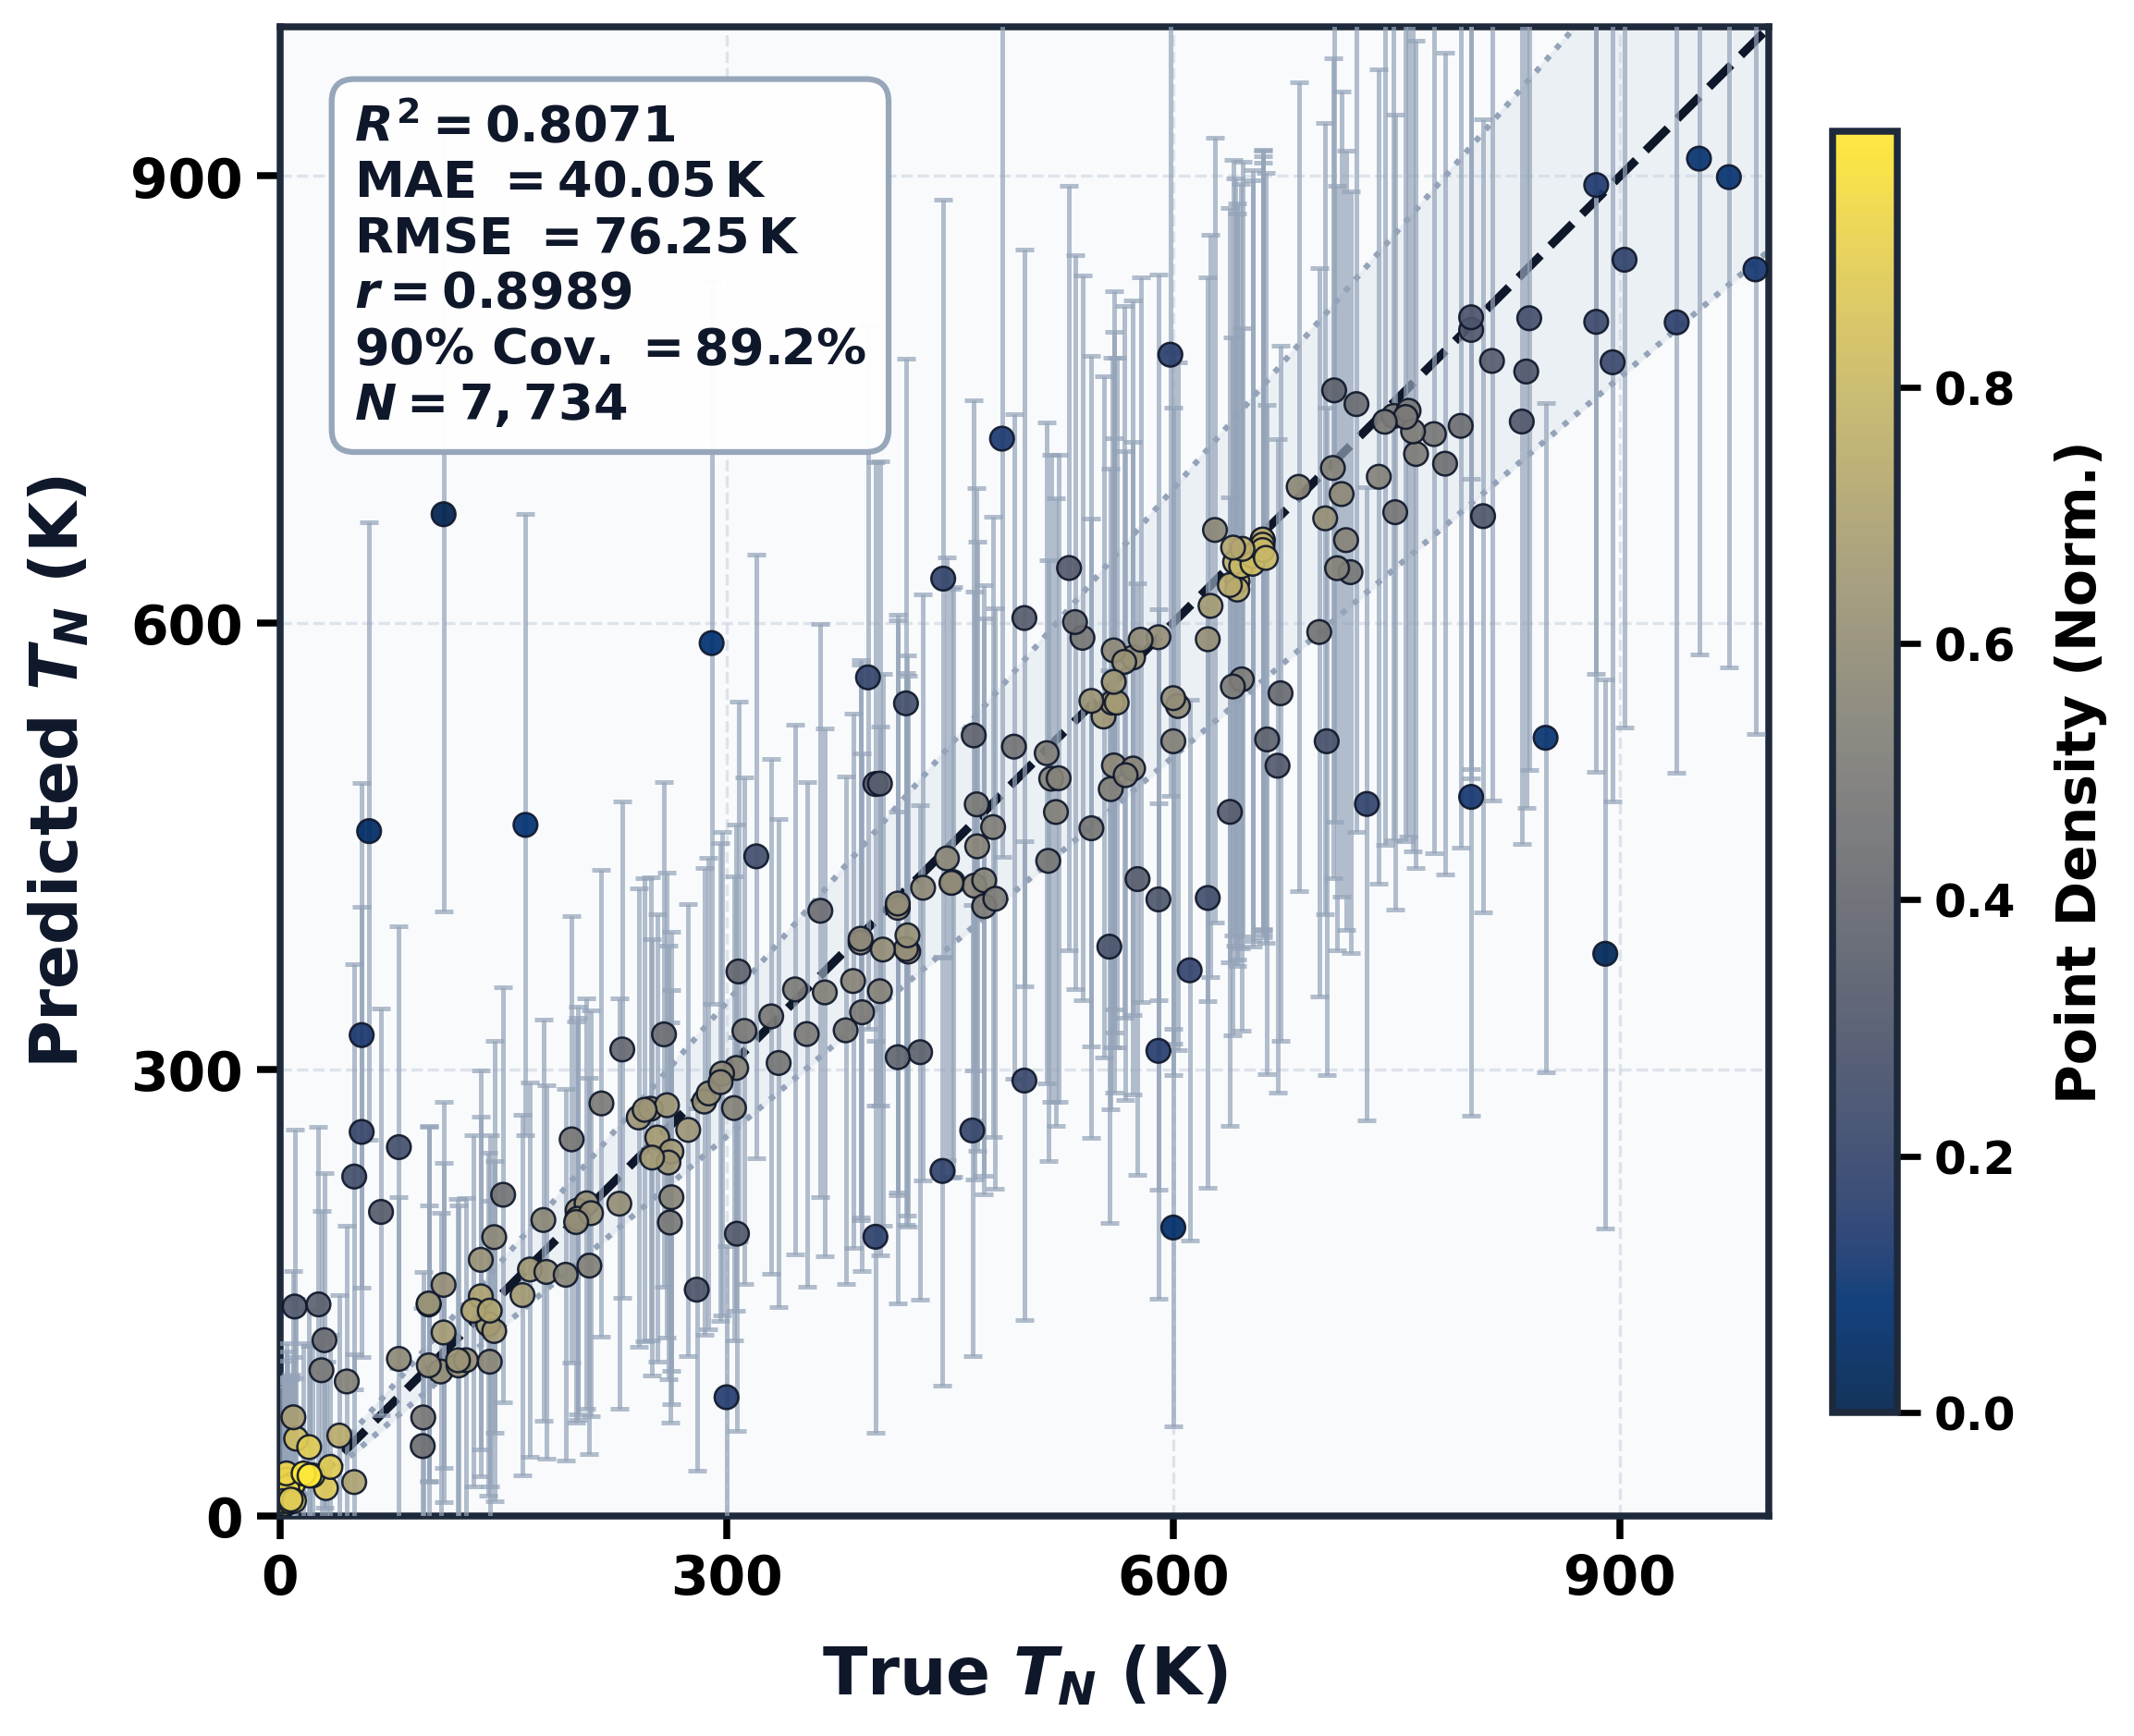
\includegraphics[width=\textwidth]{figures/neel_parity.png}
        \caption{Néel Temperature ($T_N$) Parity}
        \label{fig:neel_parity}
    \end{subfigure}
    \caption{Parity plots for Curie ($T_C$) and Néel ($T_N$) transition temperatures. Both models show strong accuracy across operating temperatures ($R^2 = 0.82$ and $0.74$), with slight scatter below 100~K.}
    \label{fig:pair_temperatures}
\end{figure}

\textbf{Magnetization and Coercivity ($M_s$ and $H_c$):} Saturation magnetization reaches $R^2 = 0.54$ ($\text{MAE} = 26.1\,\text{emu/g}$, Figure~\ref{fig:pair_moment_coercivity}). Coercivity spans four orders of magnitude ($10^2$ to $10^6\,\text{A/m}$). Because coercivity depends on grain boundaries and defects not captured by formula alone, predictions show wider scatter ($\text{MAE} = 0.65$ in $\log_{10}$ scale). Nonetheless, the overall trend ($R^2 = 0.62$) reliably separates hard from soft magnets.

\begin{figure}[!t]
    \centering
    \begin{subfigure}[b]{0.485\textwidth}
        \centering
        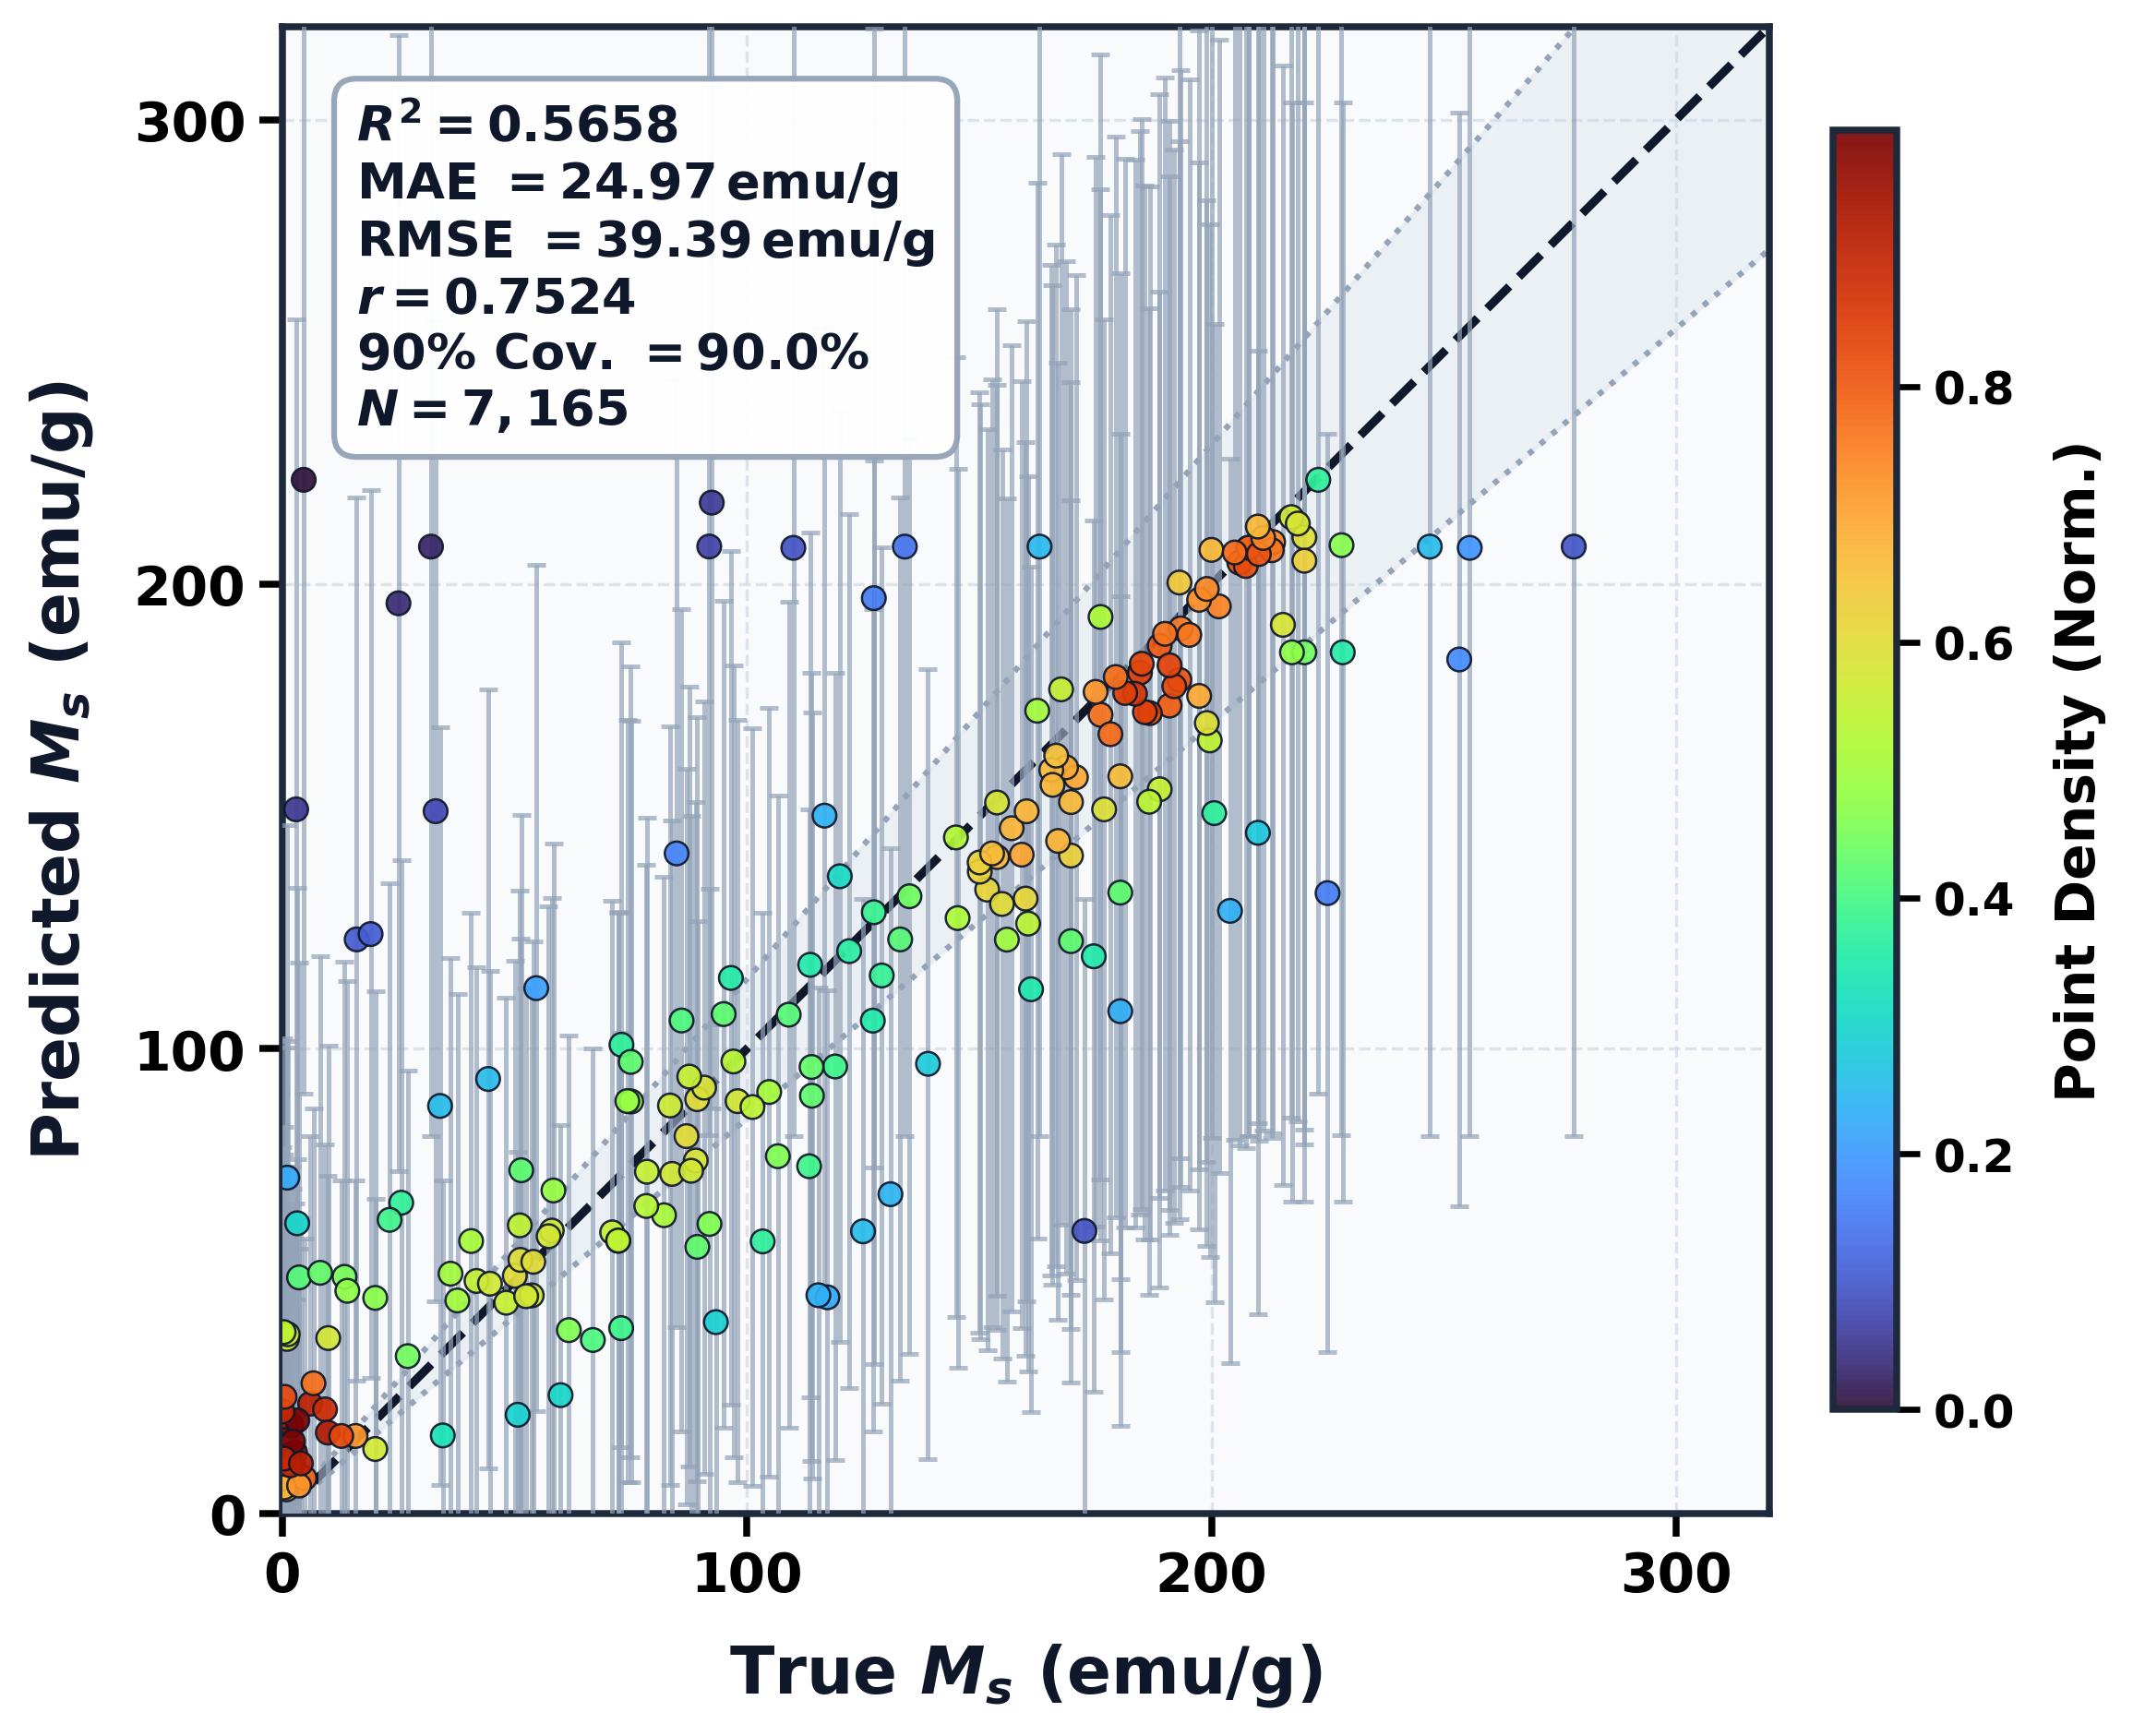
\includegraphics[width=\textwidth]{figures/magnetization_parity.png}
        \caption{Saturation Magnetization ($M_s$) Parity}
        \label{fig:ms_parity}
    \end{subfigure}
    \hfill
    \begin{subfigure}[b]{0.485\textwidth}
        \centering
        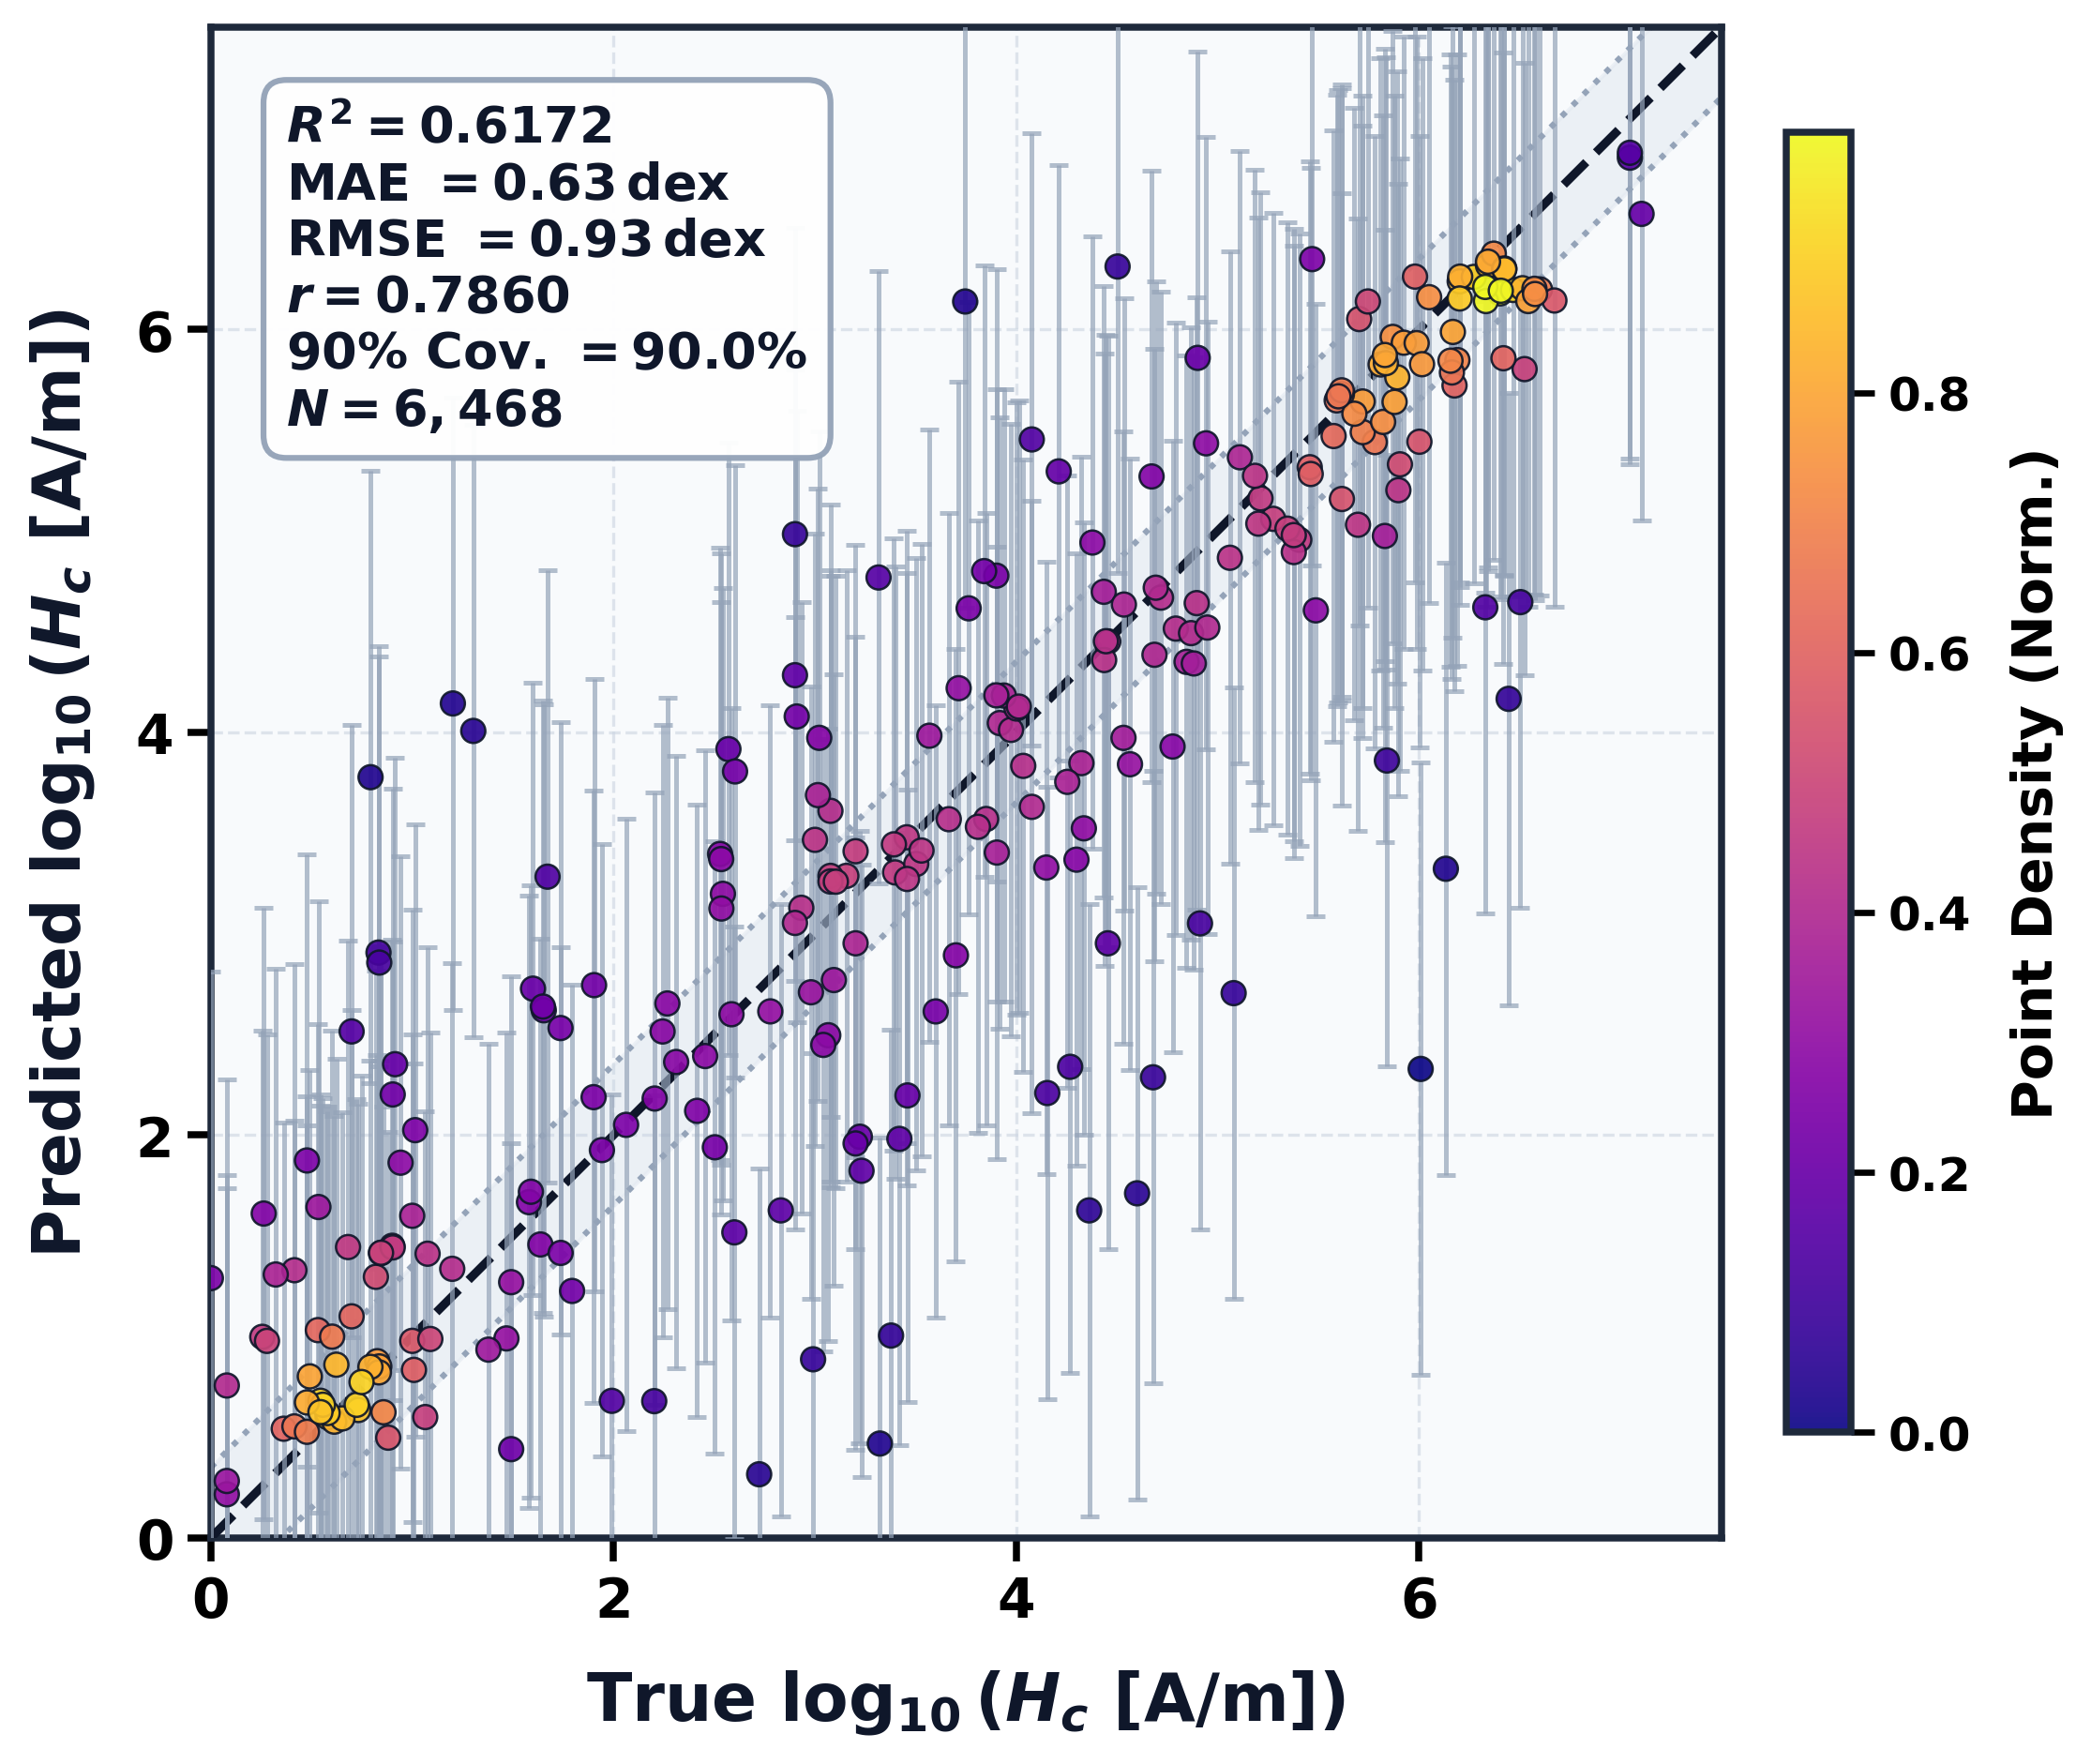
\includegraphics[width=\textwidth]{figures/coercivity_parity.png}
        \caption{Coercivity ($H_c$) Parity}
        \label{fig:hc_parity}
    \end{subfigure}
    \caption{Parity plots for saturation magnetization ($M_s$) and coercivity ($H_c$). Magnetization shows moderate predictive utility ($R^2 = 0.54$). Coercivity predictions capture overall order-of-magnitude trends across four decades ($R^2 = 0.62$, $\text{MAE} = 0.65\,\text{dex}$), serving as an effective pre-filter for hard magnetic behavior.}
    \label{fig:pair_moment_coercivity}
\end{figure}

\textbf{Anisotropy and Energy Product ($K_1$ and $(BH)_{\max}$):} Anisotropy $K_1$ ($R^2 = 0.46$, Figure~\ref{fig:pair_anisotropy_bhmax}) identifies strong easy-axis candidates ($K_1 > 10^6\,\text{J/m}^3$). For energy product $(BH)_{\max}$ ($R^2 = 0.51$, $\text{MAE} = 0.27$ in $\log_{10}$ scale), the cascade enforces $(BH)_{\max} \le \frac{1}{4}\mu_0 M_s^2$, preventing unphysical predictions.

\begin{figure}[!t]
    \centering
    \begin{subfigure}[b]{0.485\textwidth}
        \centering
        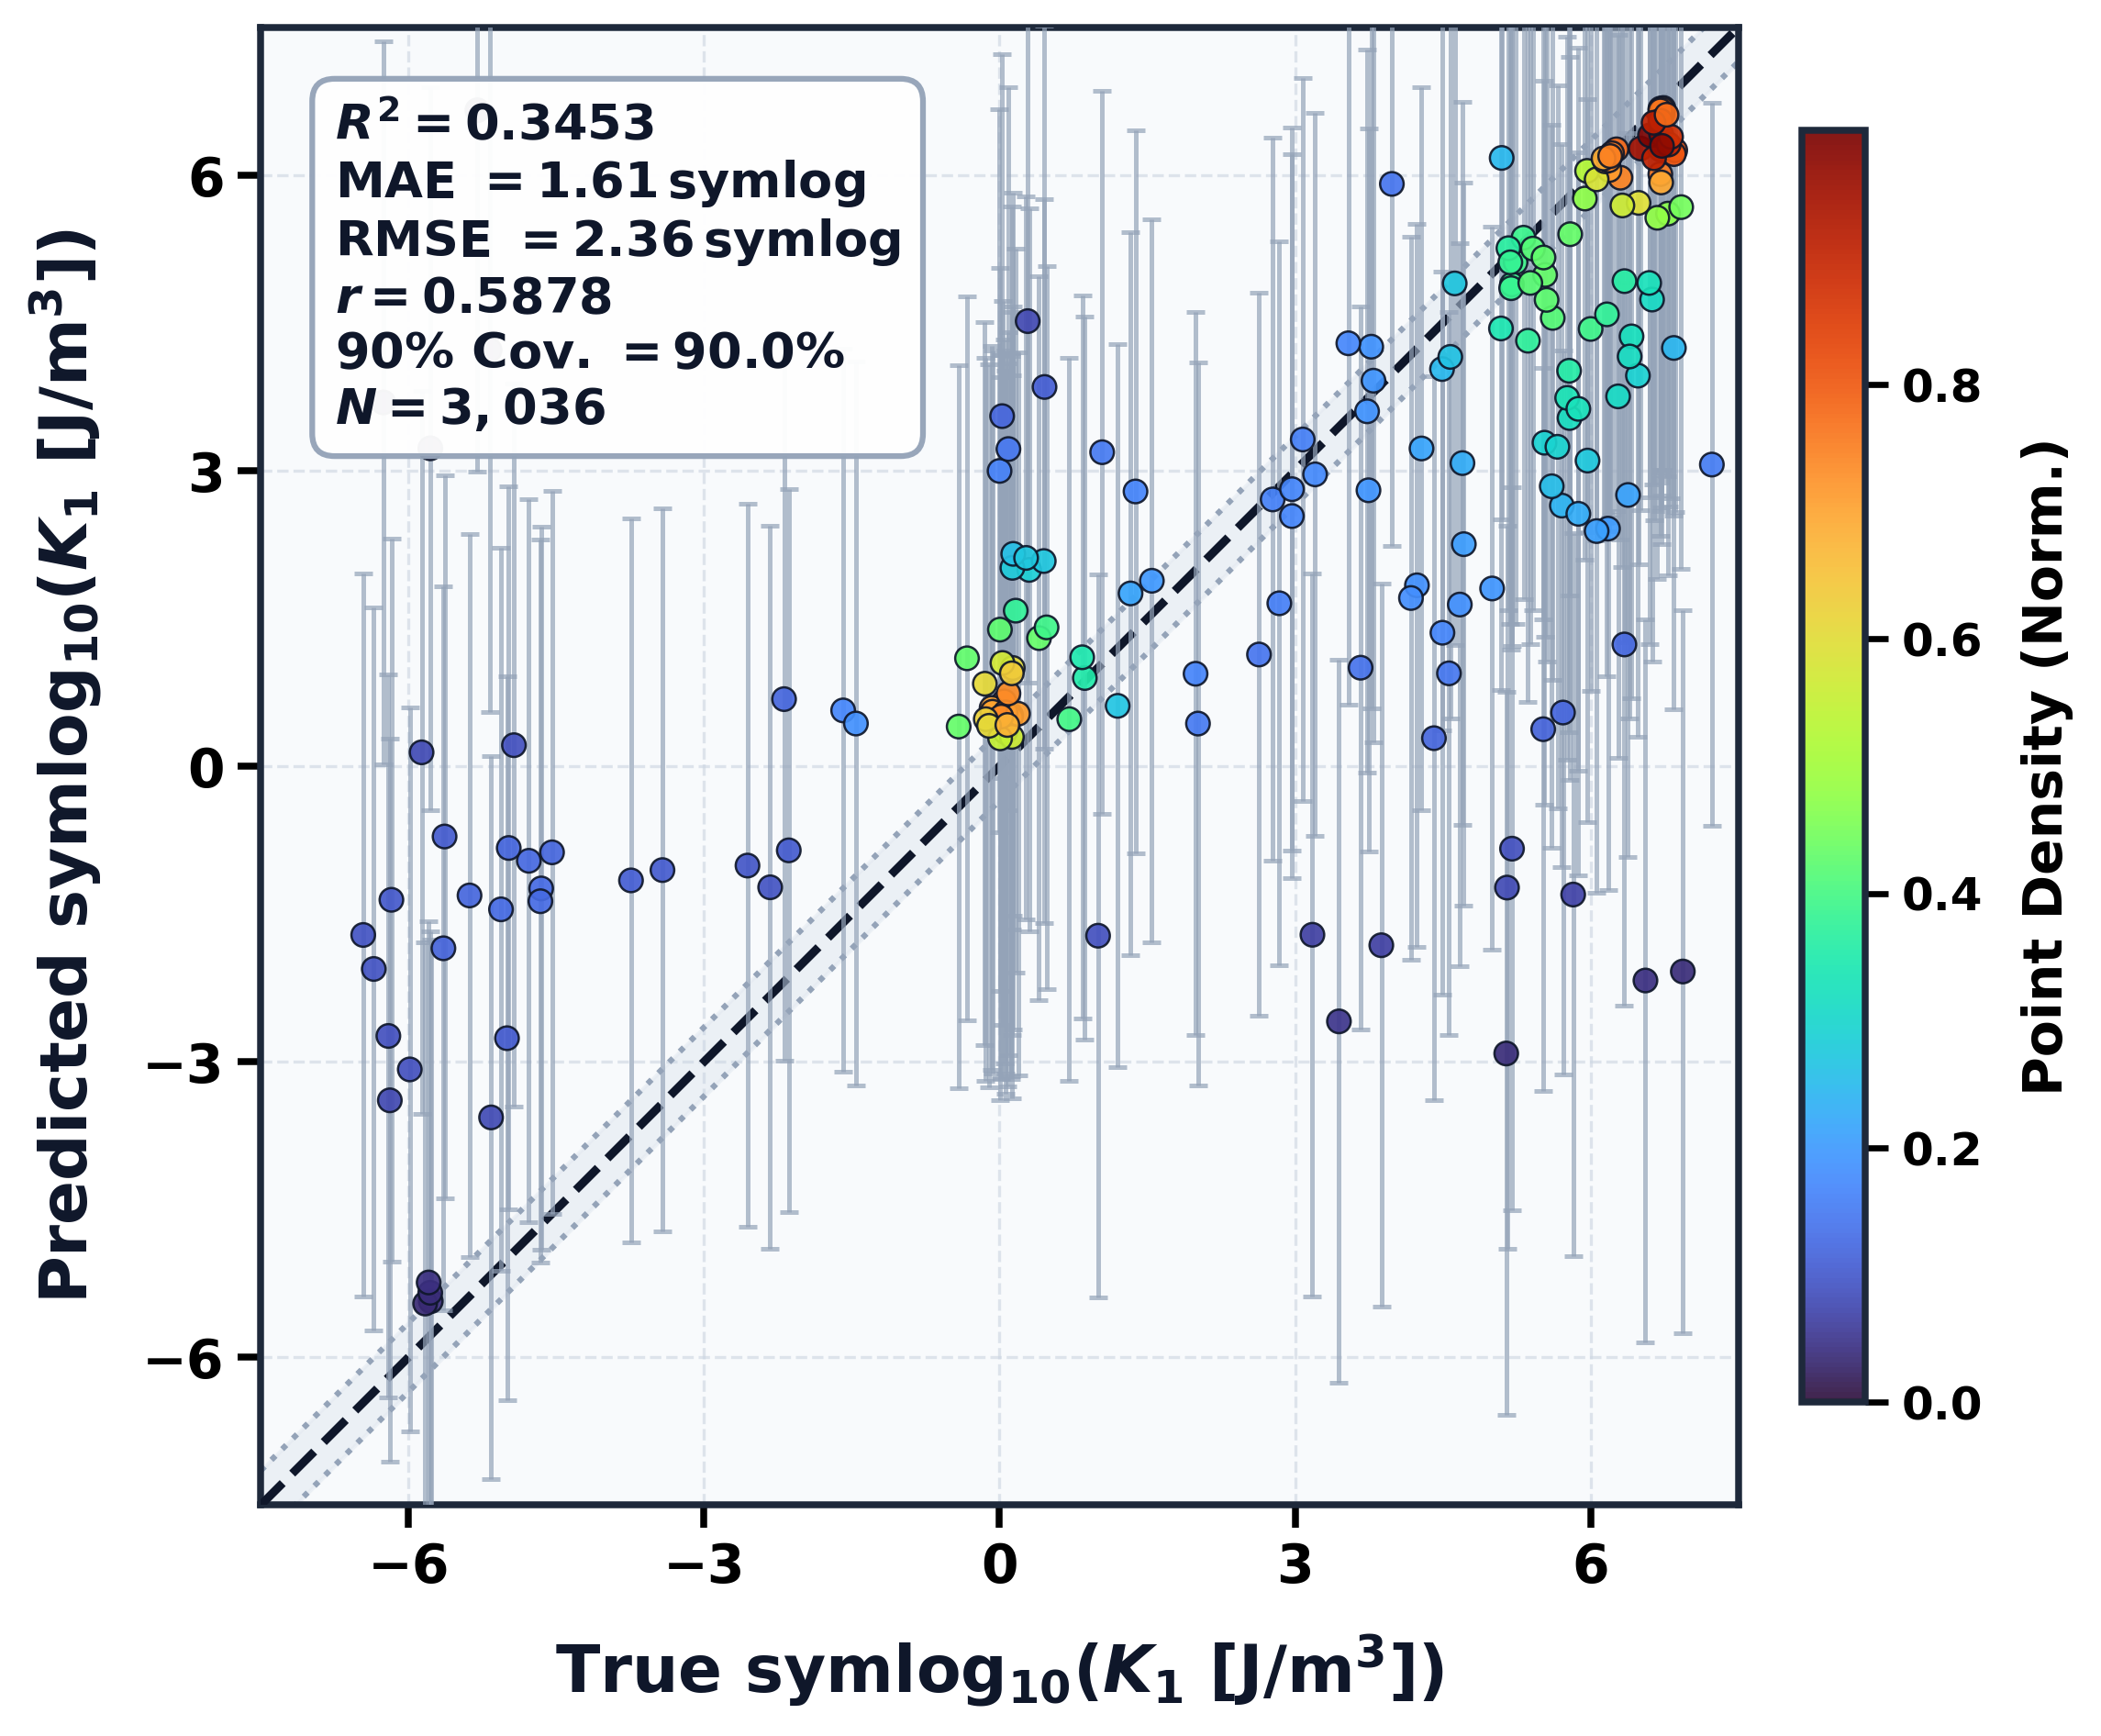
\includegraphics[width=\textwidth]{figures/anisotropy_parity.png}
        \caption{Anisotropy Constant ($K_1$) Parity}
        \label{fig:k1_parity}
    \end{subfigure}
    \hfill
    \begin{subfigure}[b]{0.485\textwidth}
        \centering
        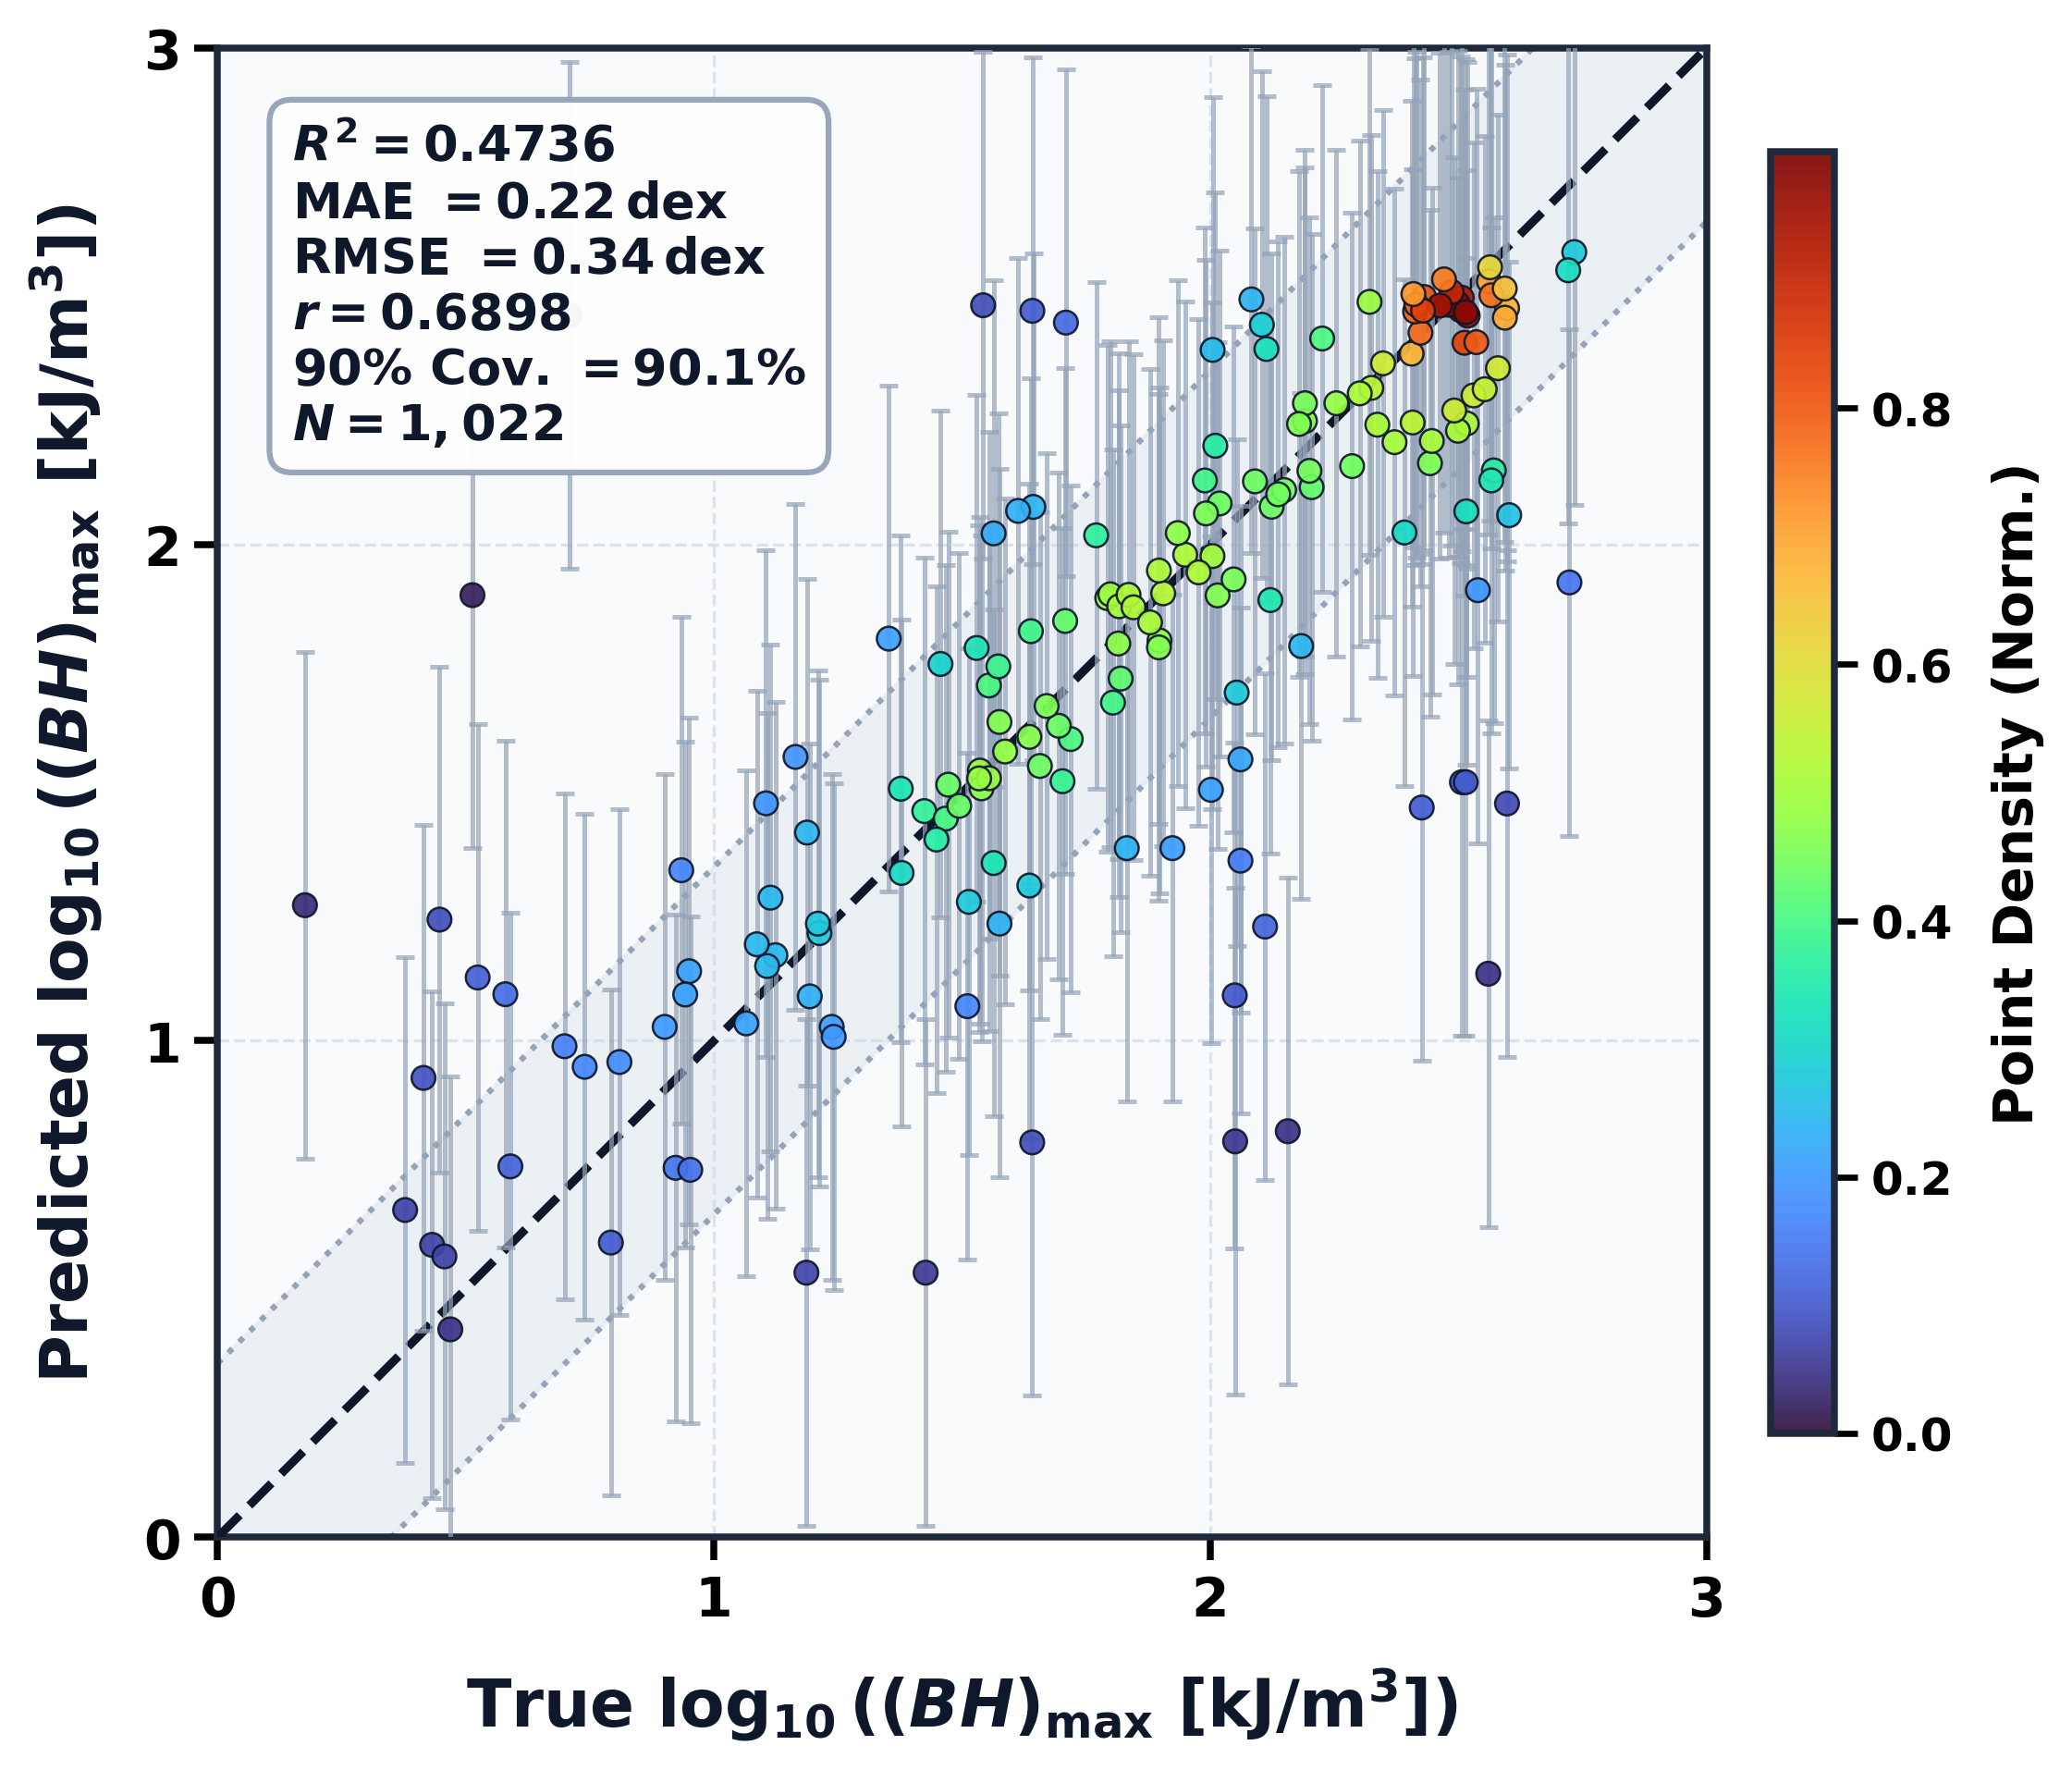
\includegraphics[width=\textwidth]{figures/bh_max_parity.png}
        \caption{Energy Product ($(BH)_{\max}$) Parity}
        \label{fig:bhmax_parity}
    \end{subfigure}
    \caption{Parity plots for magnetocrystalline anisotropy ($K_1$) and maximum energy product ($(BH)_{\max}$). Cascade modeling ensures $(BH)_{\max}$ remains within thermodynamic limits. The moderate scores ($R^2 = 0.46$ and $0.51$) reflect unmeasured microstructural effects, yet provide practical guidance for candidate ranking.}
    \label{fig:pair_anisotropy_bhmax}
\end{figure}

\subsection{Manifolds, Diagnostics, and Screening}
\label{sec:diagnostics_and_screening}

To assess representation quality, classification discrimination, statistical uncertainty, and practical candidate discovery:

\textbf{Learned Representations and Micromagnetic Scaling:} Figure~\ref{fig:pair_umap_kronmuller}(a) maps MagFormer features via UMAP, showing distinct clusters for ferromagnetic, antiferromagnetic, and non-magnetic materials. Figure~\ref{fig:pair_umap_kronmuller}(b) confirms that coercivity scales with the Kronmüller parameter ($2K_1 / \mu_0 M_s$).

\begin{figure}[!t]
    \centering
    \begin{subfigure}[b]{0.485\textwidth}
        \centering
        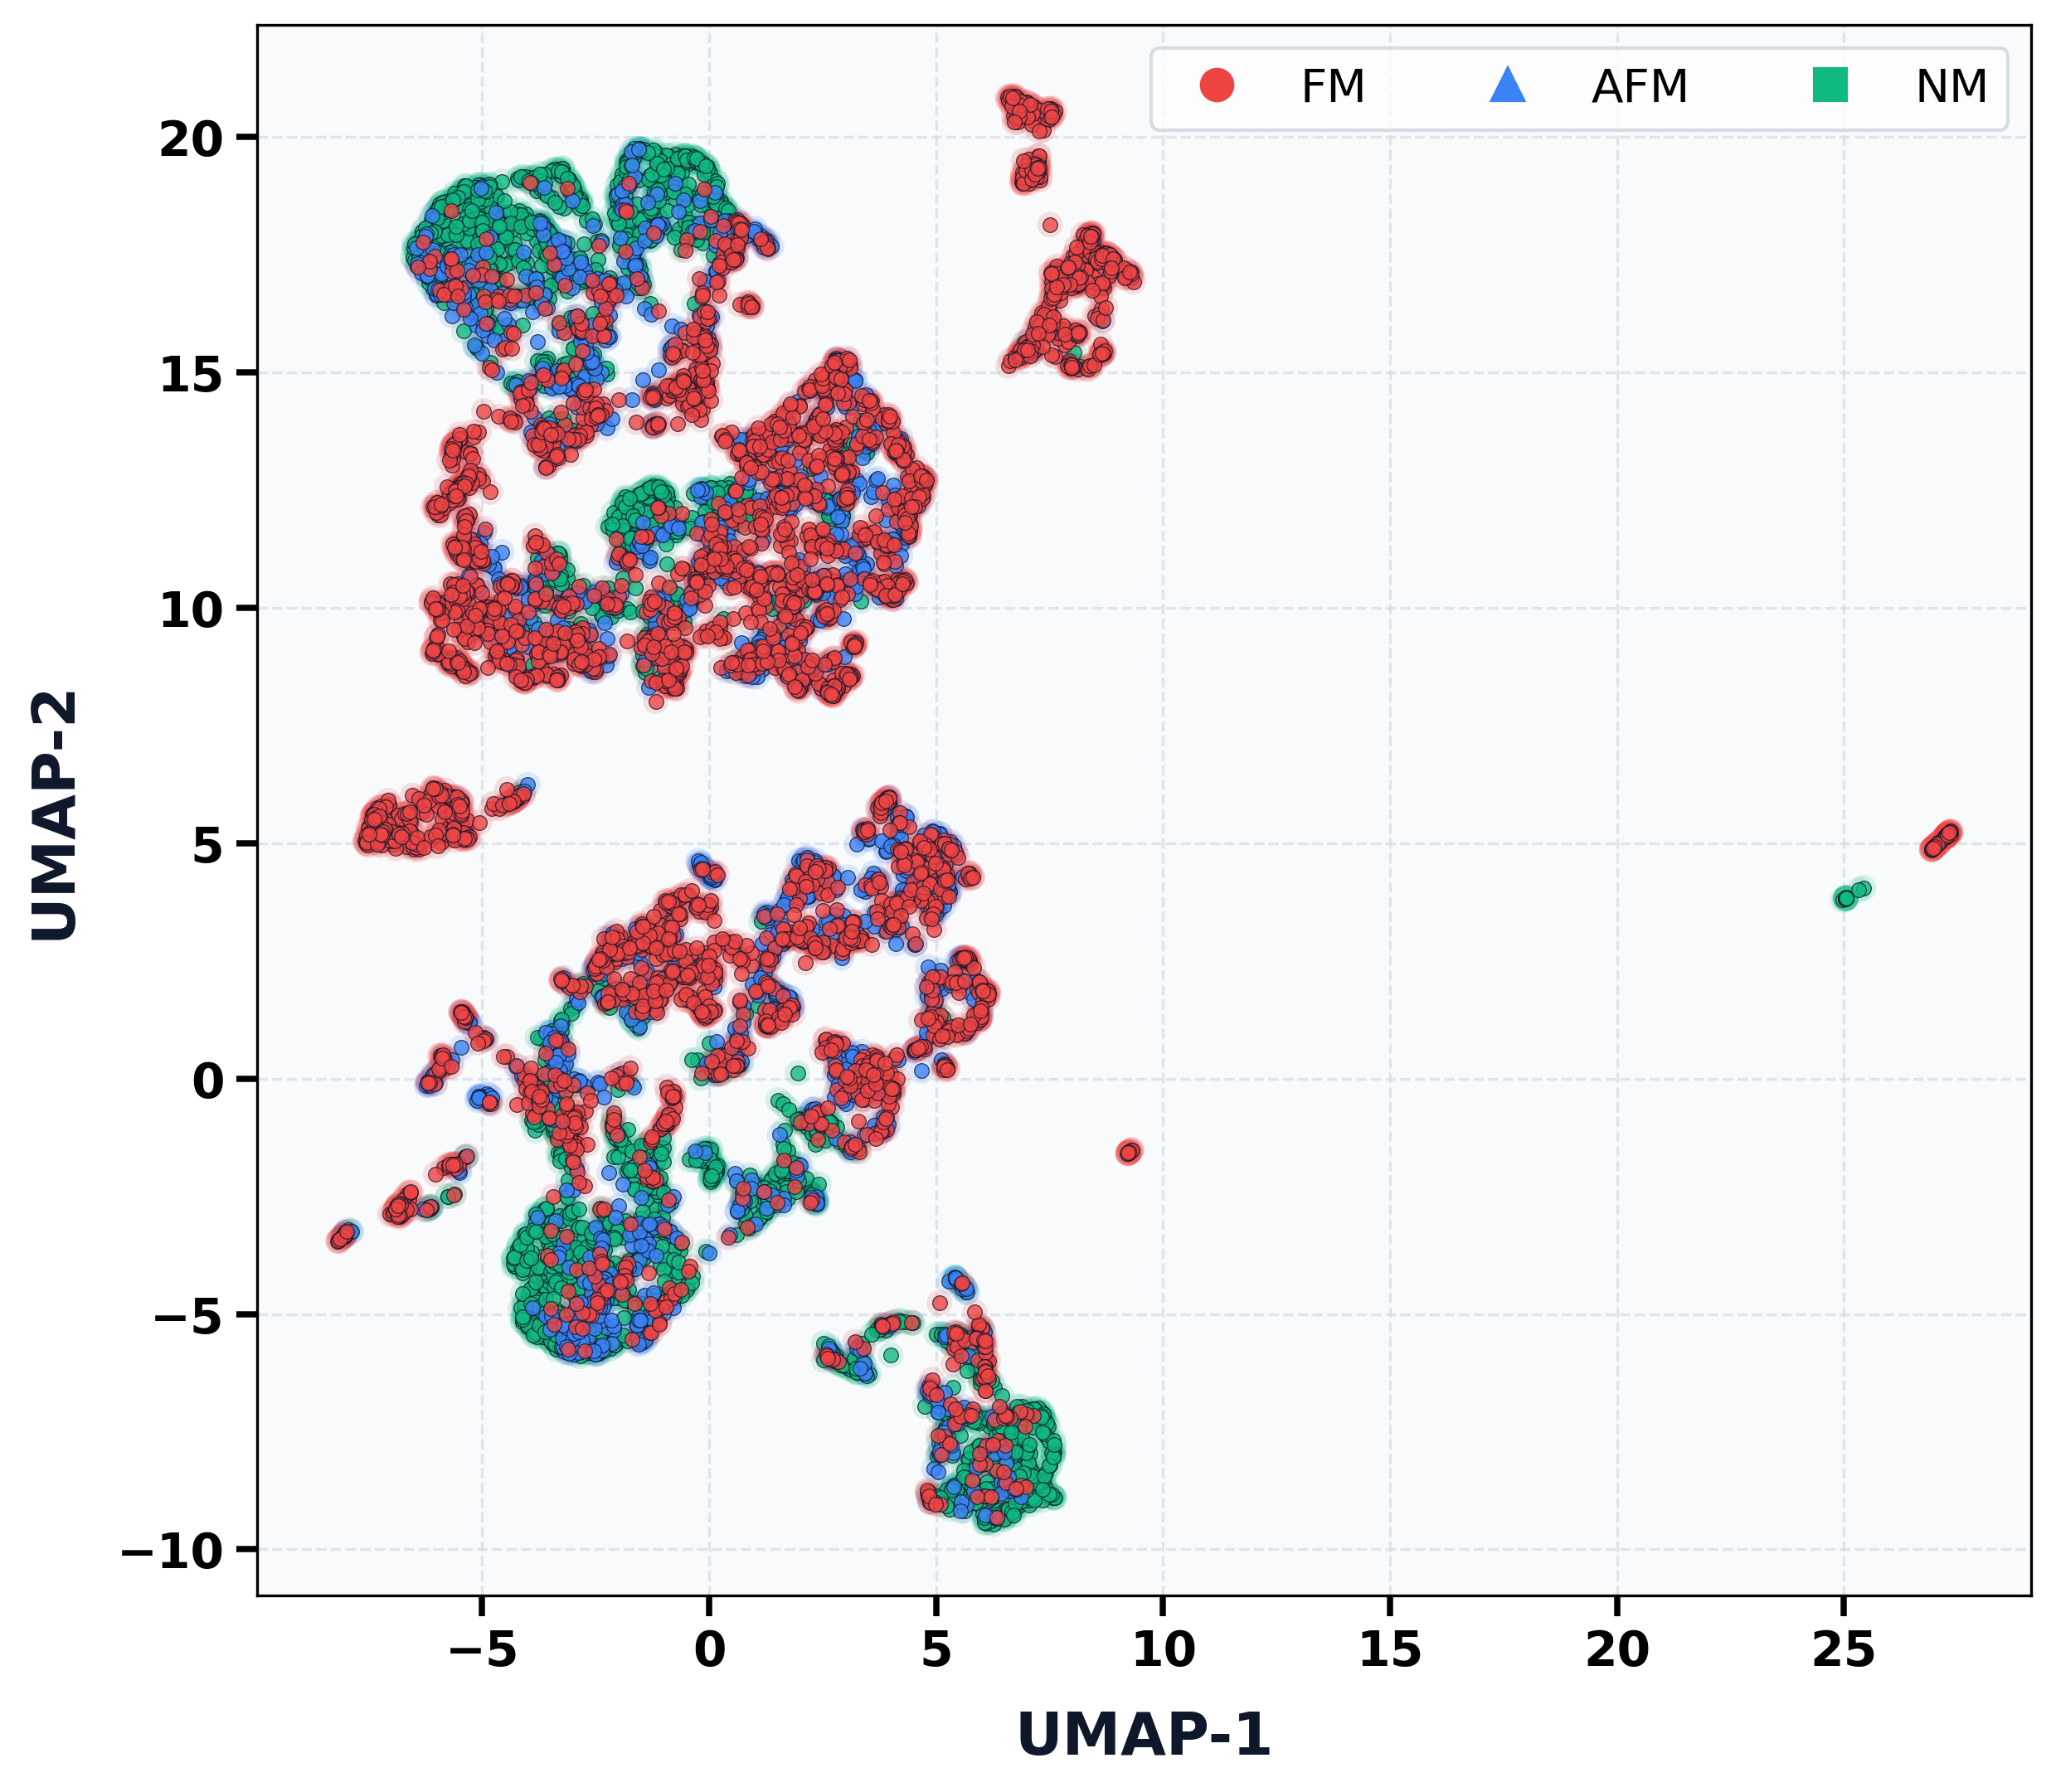
\includegraphics[width=\textwidth]{figures/latent_manifold_umap.png}
        \caption{Latent Representation Manifold (UMAP)}
        \label{fig:umap_manifold}
    \end{subfigure}
    \hfill
    \begin{subfigure}[b]{0.485\textwidth}
        \centering
        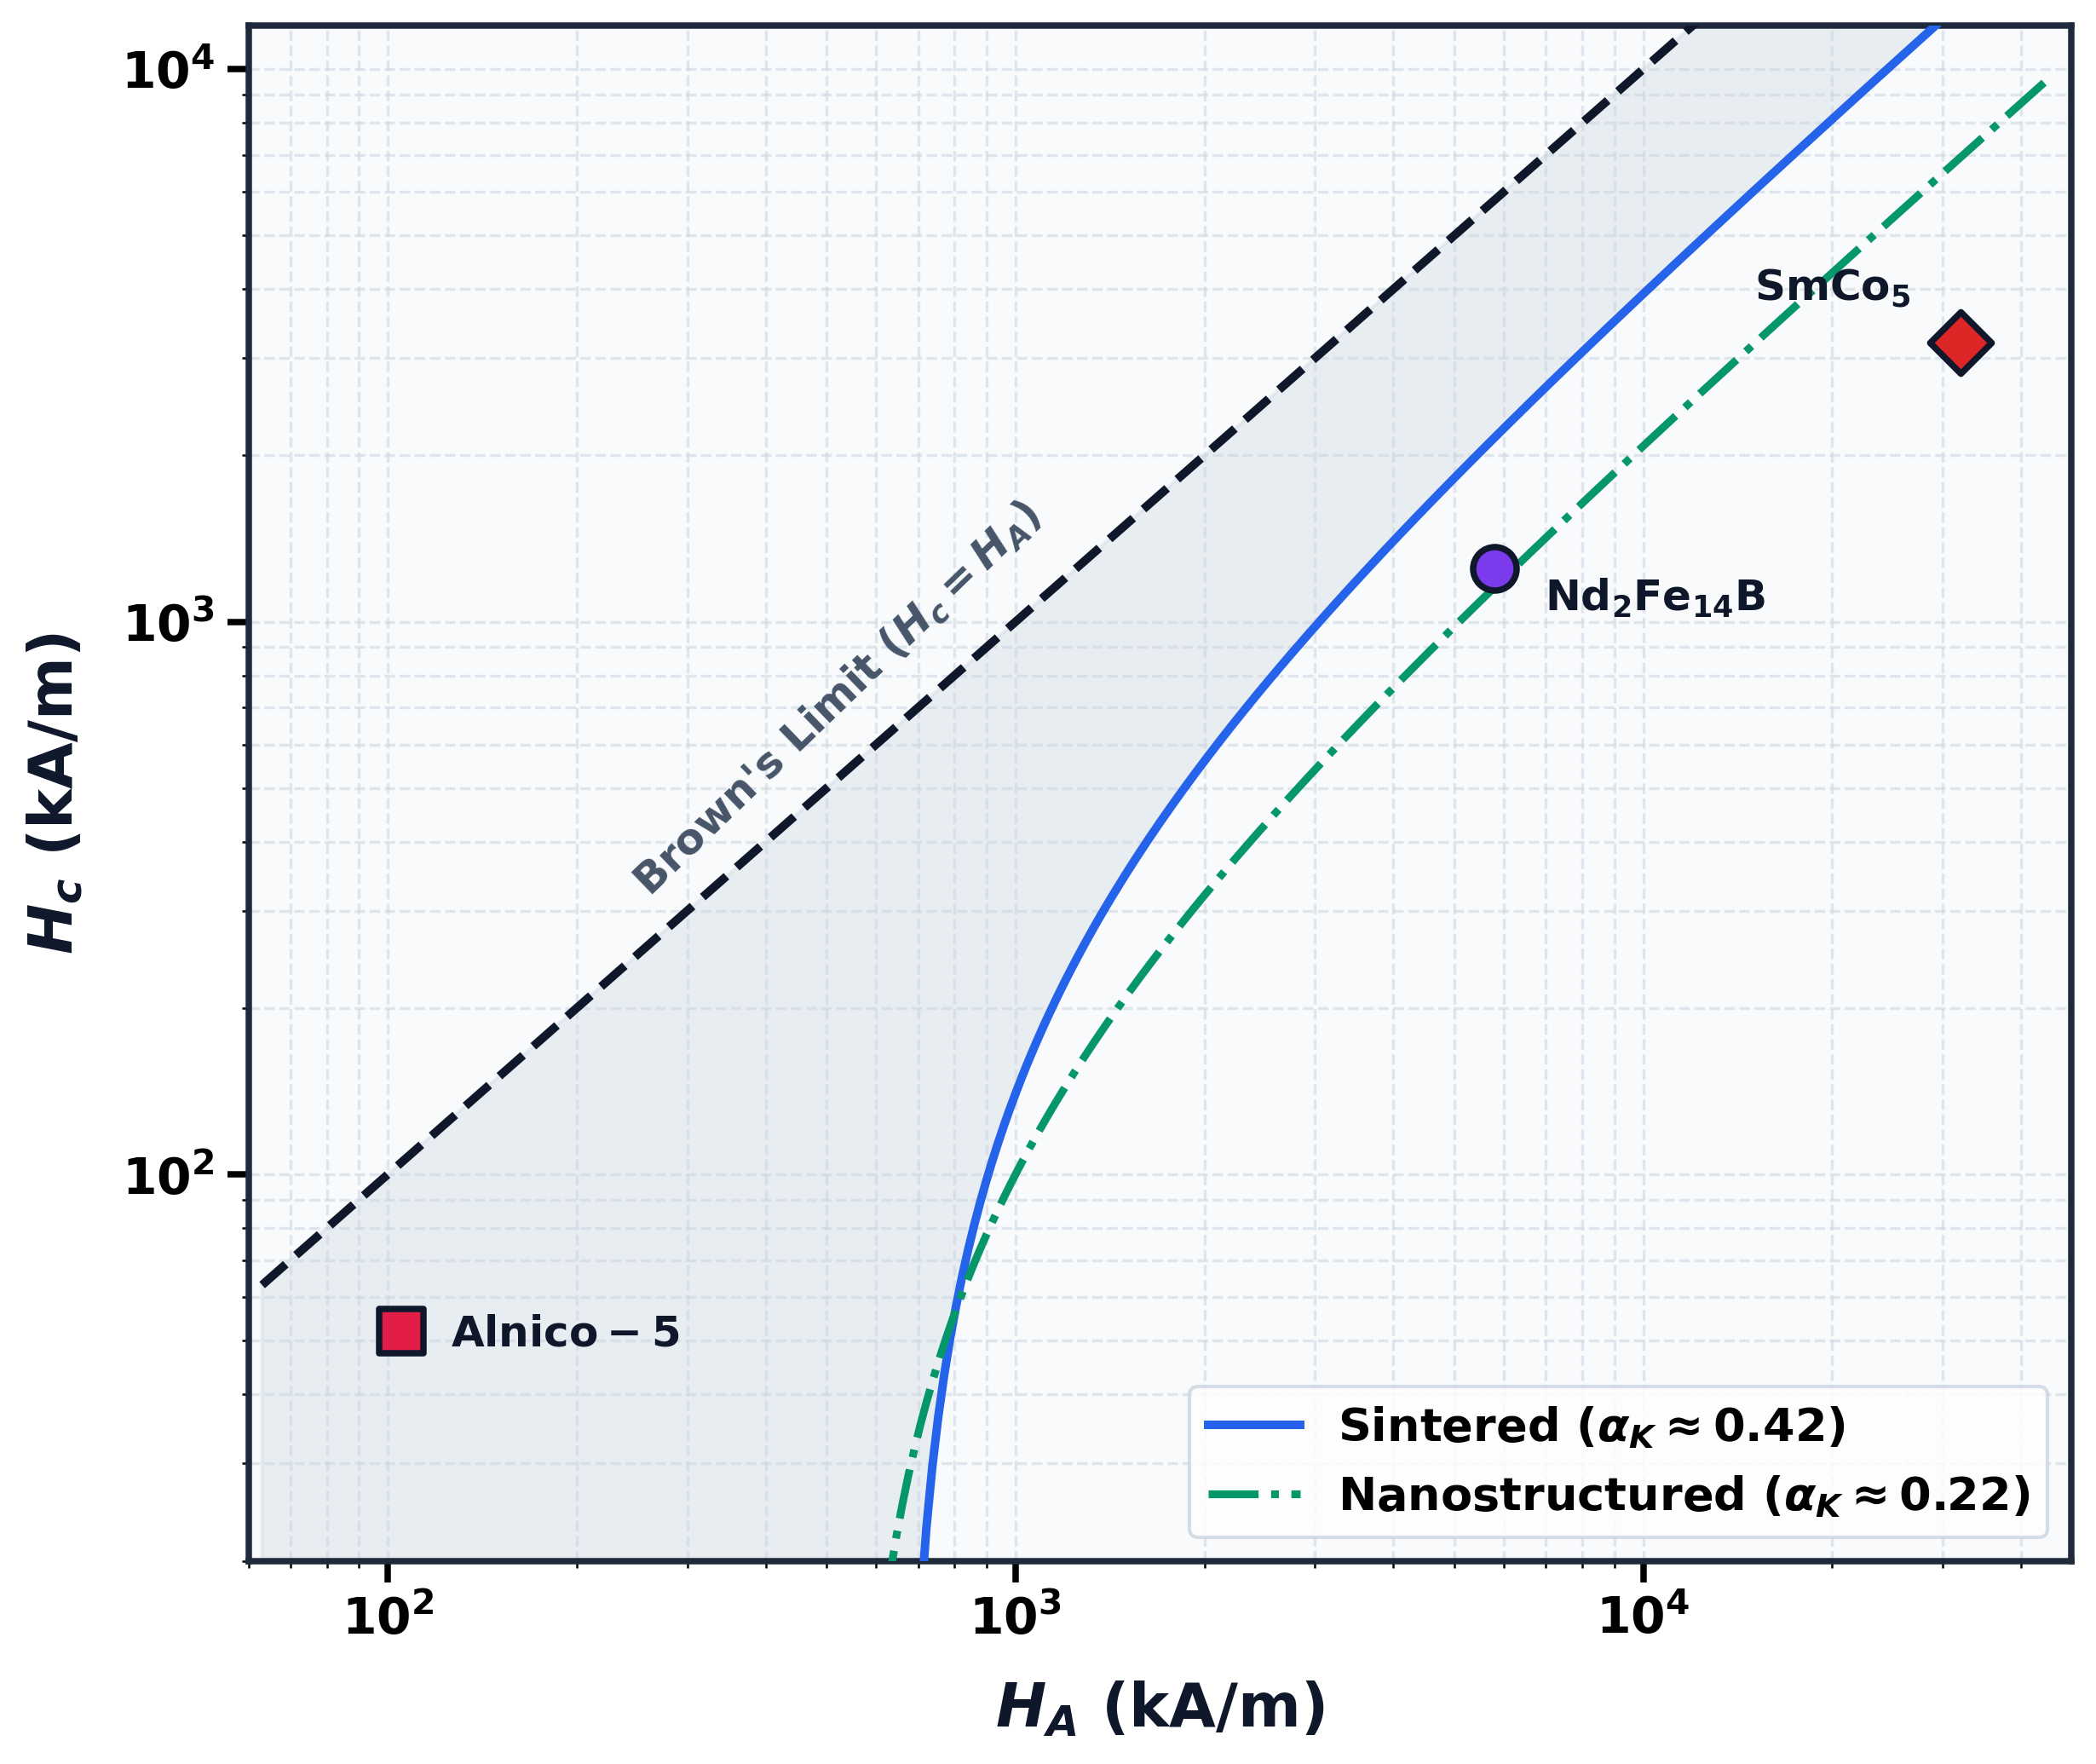
\includegraphics[width=\textwidth]{figures/kronmuller_micromagnetic_analysis.png}
        \caption{Kronmüller Micromagnetic Coercivity Scaling}
        \label{fig:kronmuller_plot}
    \end{subfigure}
    \caption{Latent representations and micromagnetic validation. (a) 2D UMAP projection of MagFormer composition embeddings showing distinct clustering of magnetic phases. (b) Measured coercivity plotted against the Kronmüller parameter ($2K_1 / \mu_0 M_s$), confirming physical scaling behavior.}
    \label{fig:pair_umap_kronmuller}
\end{figure}

\textbf{Magnetic Phase Classification:} Phase classification achieves 91.9\% accuracy ($\text{AUC} \ge 0.96$, Figure~\ref{fig:pair_phase_roc}), with the boundary classifier reaching $F_1 = 0.82$ on the smaller antiferromagnetic class.

\begin{figure}[!t]
    \centering
    \begin{subfigure}[b]{0.485\textwidth}
        \centering
        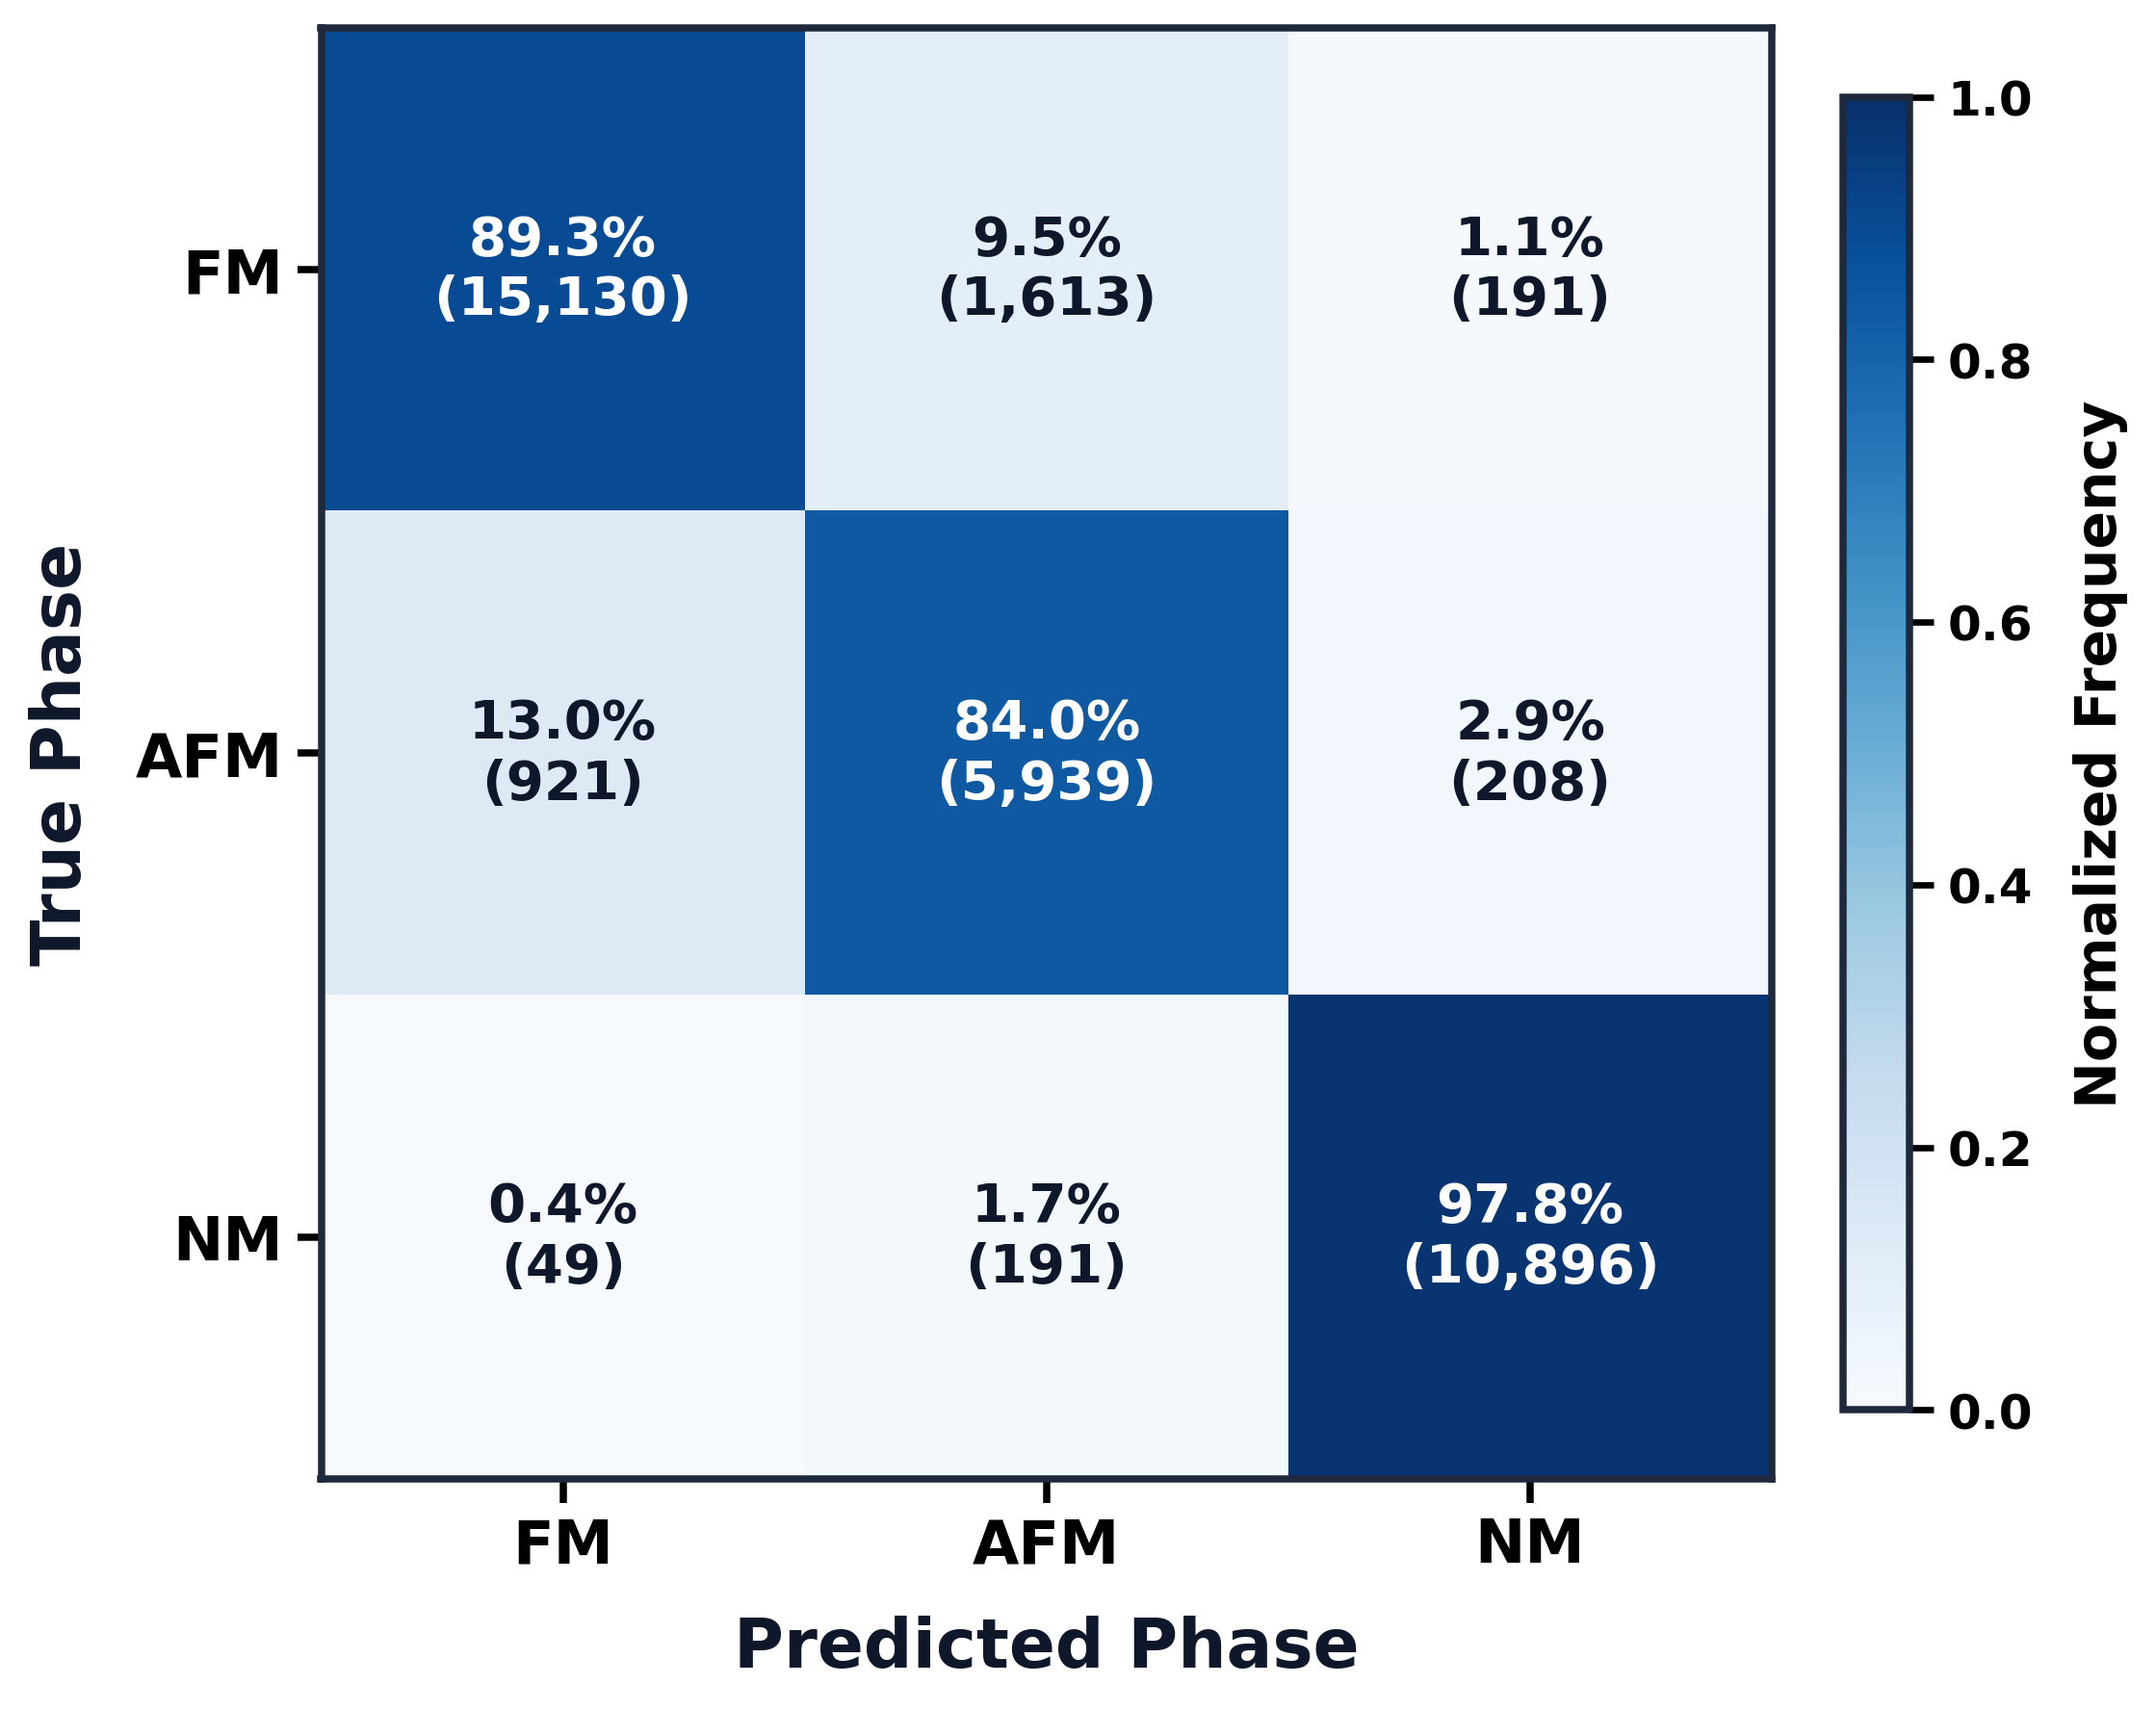
\includegraphics[width=\textwidth]{figures/phase_confusion_matrix.png}
        \caption{Phase Confusion Matrix}
        \label{fig:confusion_matrix}
    \end{subfigure}
    \hfill
    \begin{subfigure}[b]{0.485\textwidth}
        \centering
        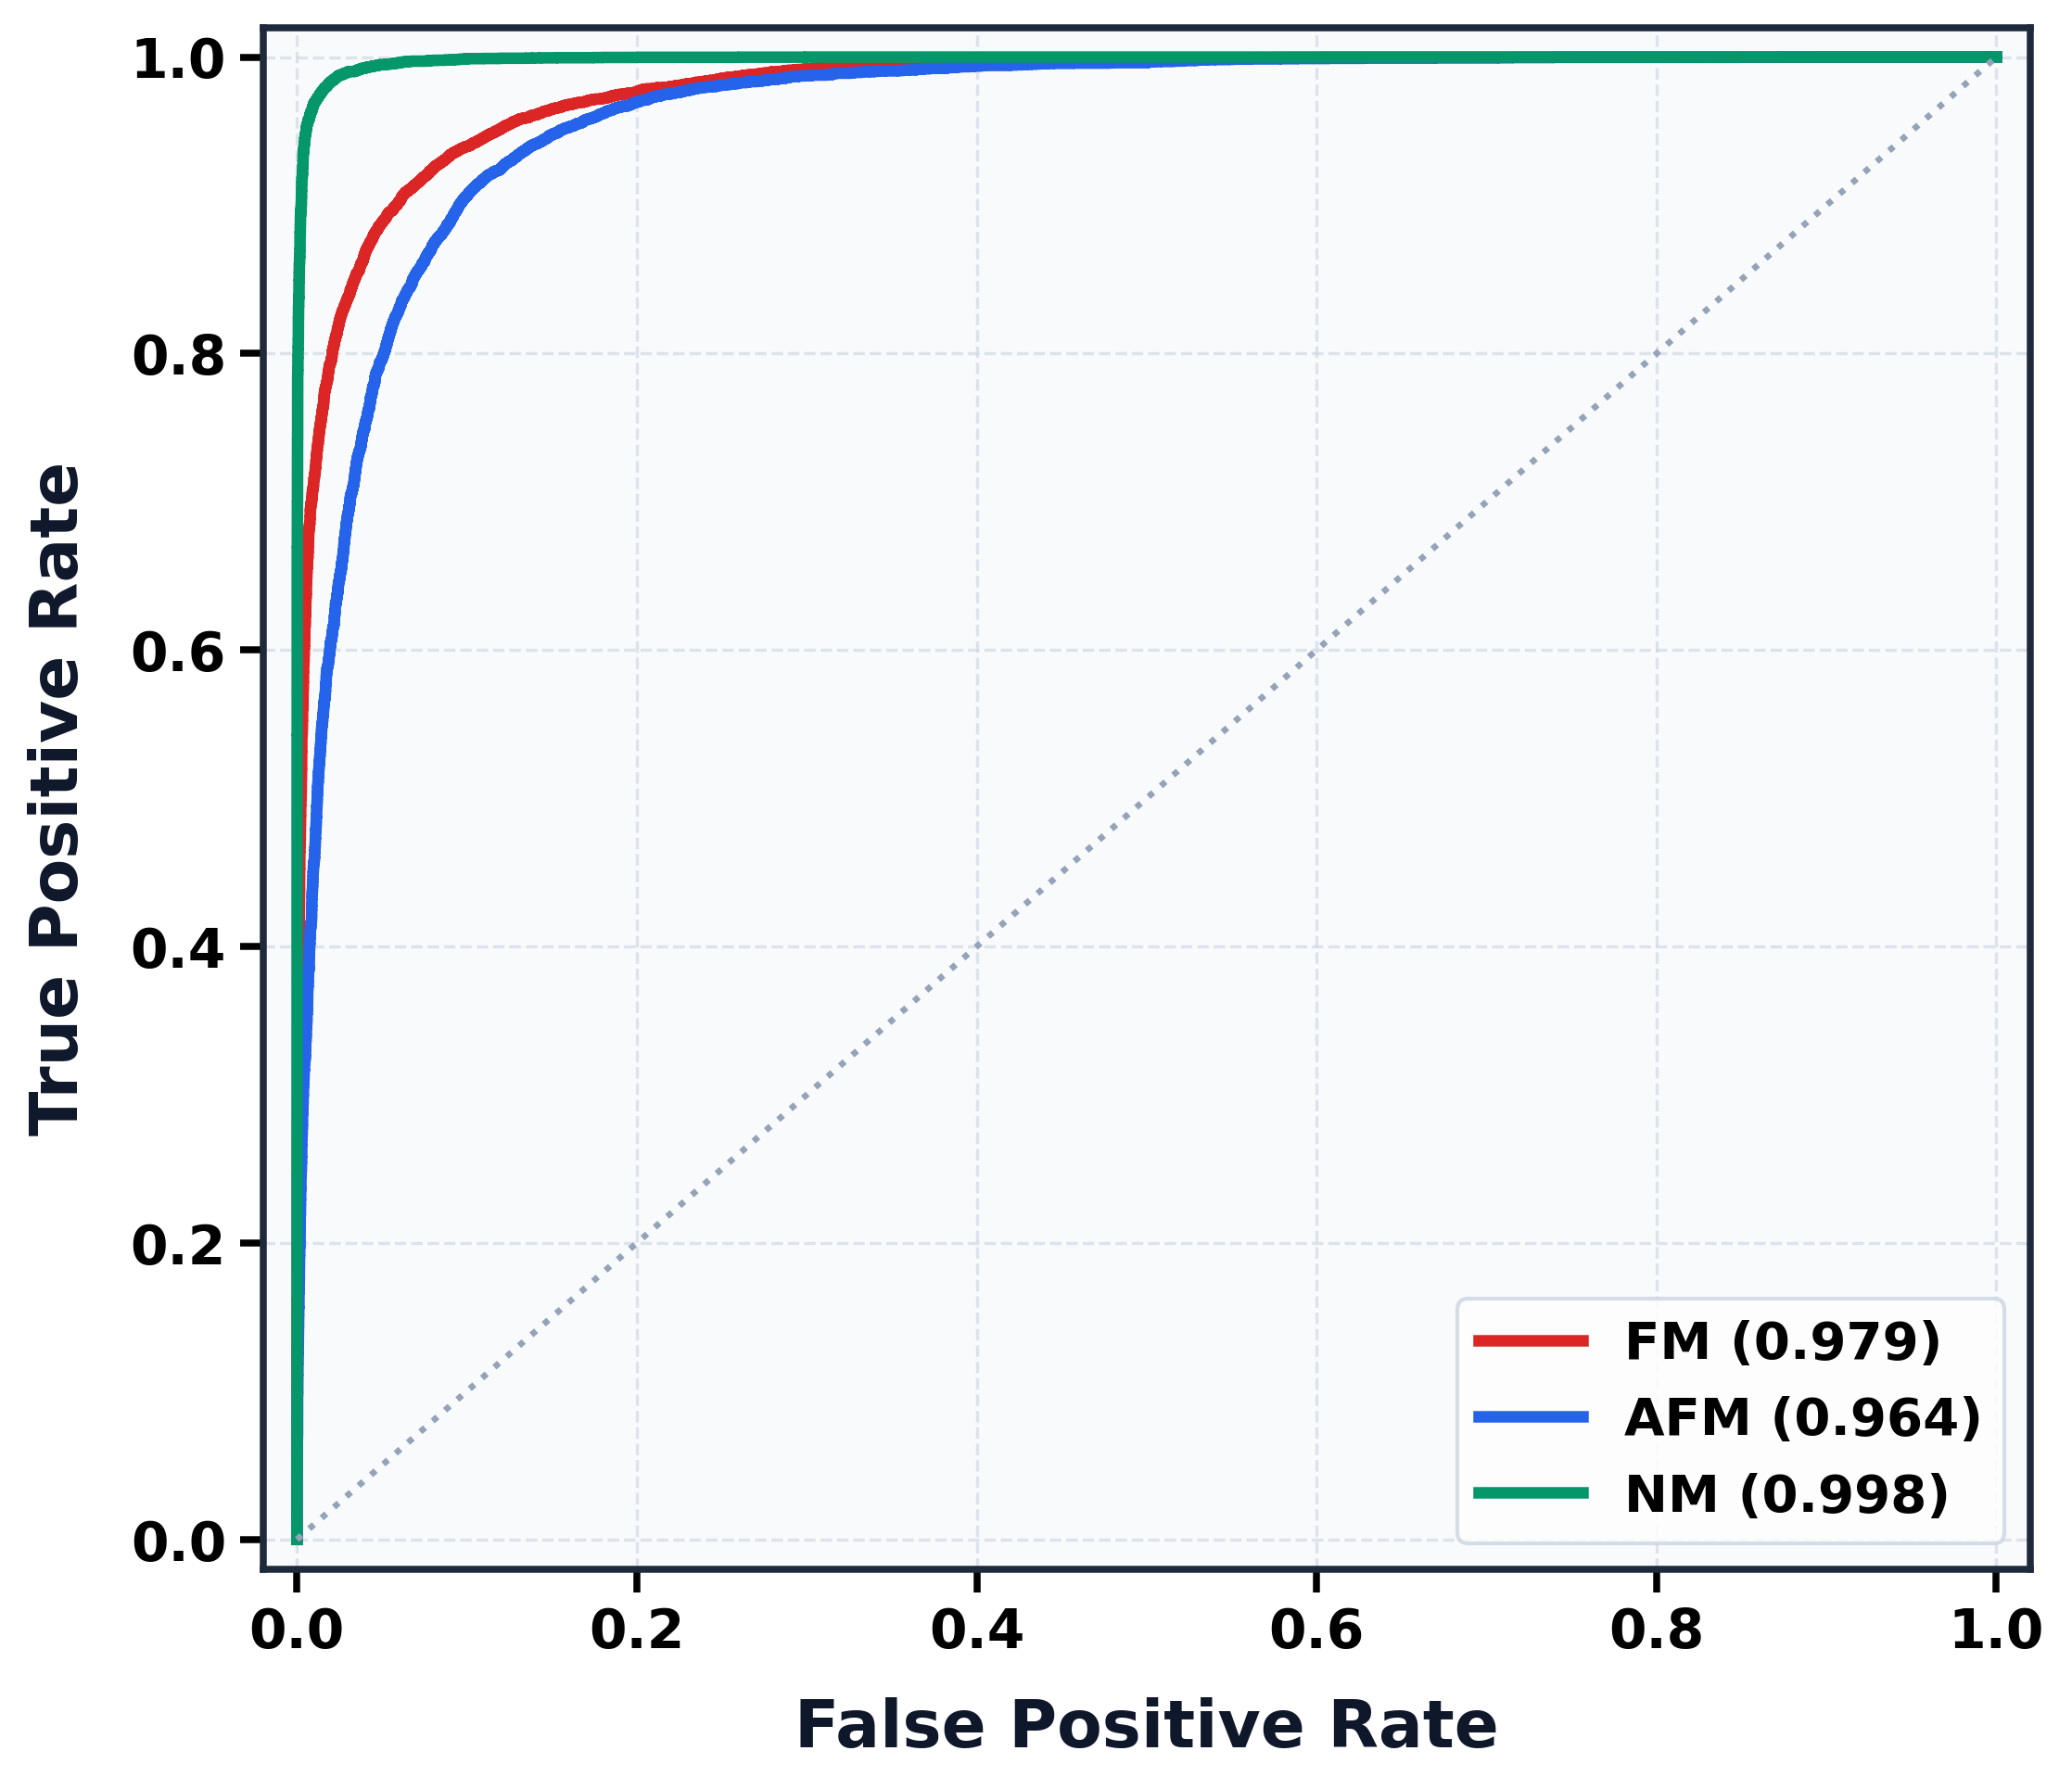
\includegraphics[width=\textwidth]{figures/phase_roc_curves.png}
        \caption{Multiclass Phase ROC Curves}
        \label{fig:roc_curves}
    \end{subfigure}
    \caption{Ground-state magnetic phase classification diagnostics. (a) Confusion matrix showing balanced discrimination across phases. (b) Multiclass ROC curves demonstrating strong discriminative ability ($\text{AUC} \ge 0.96$) across Ferromagnetic, Antiferromagnetic, and Non-magnetic classes.}
    \label{fig:pair_phase_roc}
\end{figure}

\textbf{Uncertainty Calibration:} The conformal calibration curve (Figure~\ref{fig:pair_conformal_residuals}(a)) closely tracks the ideal diagonal, confirming that 90\% intervals achieve correct coverage. Residuals remain centered near zero across operating temperatures (Figure~\ref{fig:pair_conformal_residuals}(b)).

\begin{figure}[!t]
    \centering
    \begin{subfigure}[b]{0.485\textwidth}
        \centering
        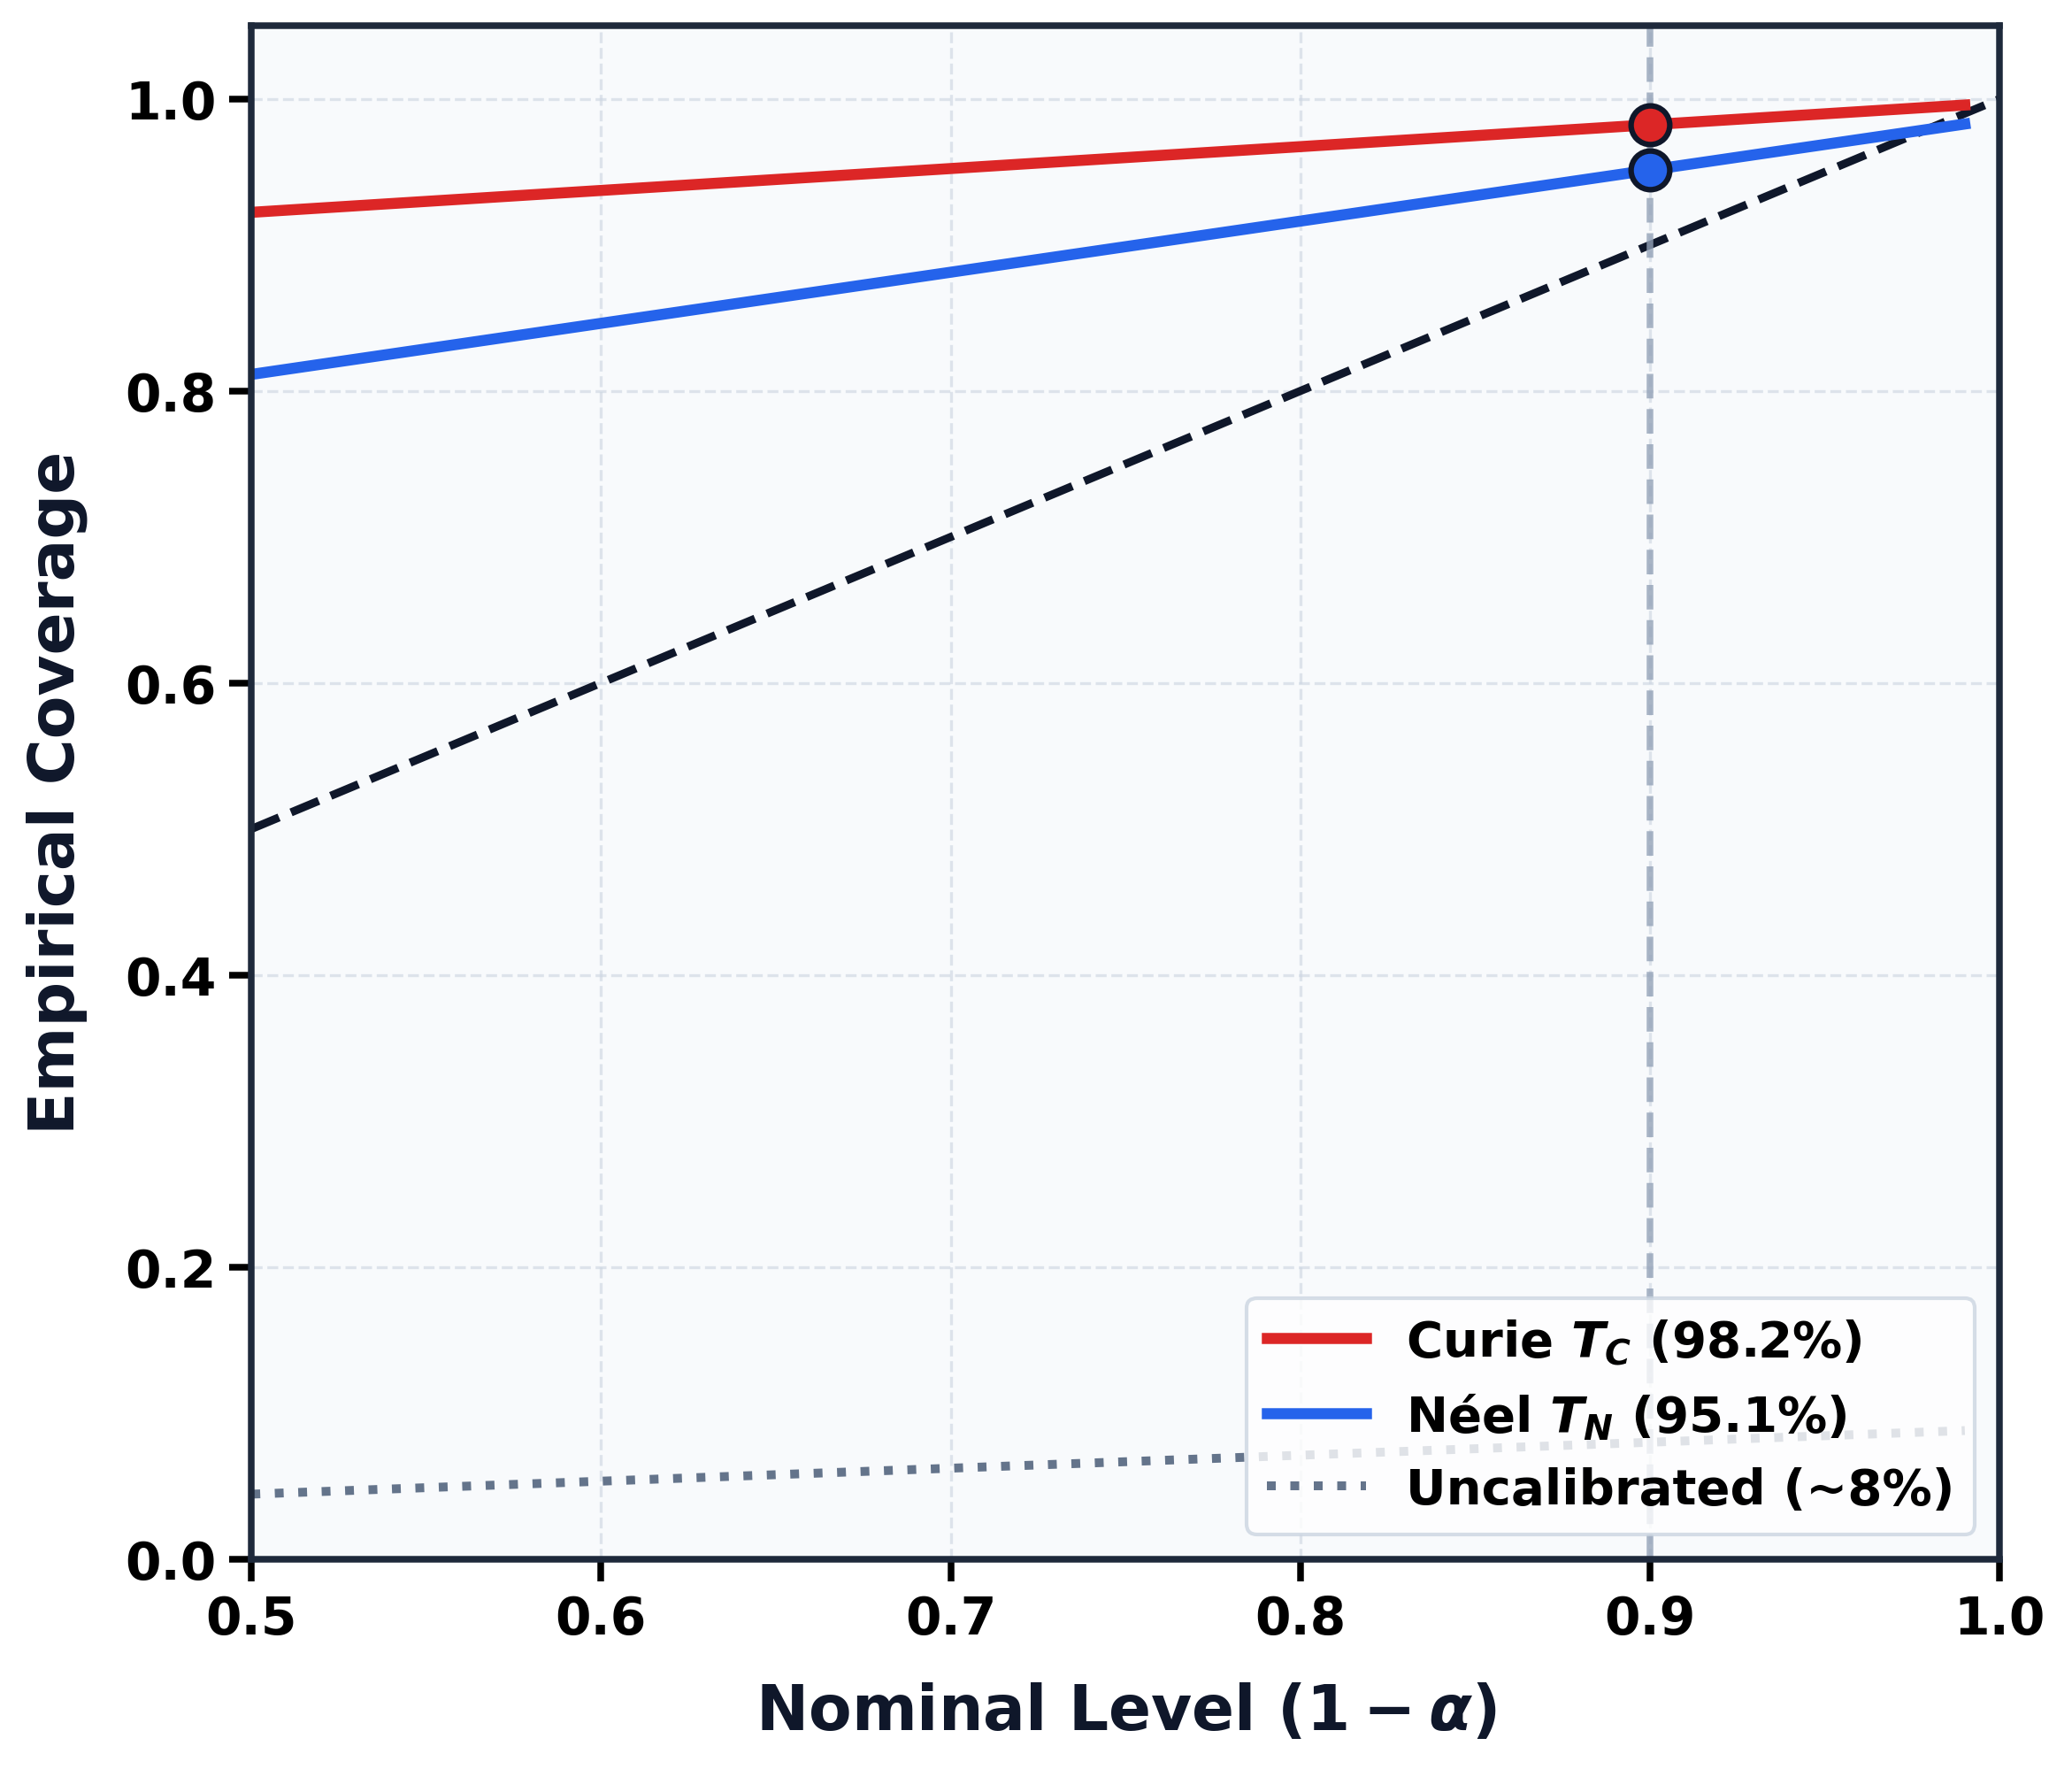
\includegraphics[width=\textwidth]{figures/conformal_calibration_curve.png}
        \caption{Conformal Calibration Coverage Curve}
        \label{fig:conformal_curve}
    \end{subfigure}
    \hfill
    \begin{subfigure}[b]{0.485\textwidth}
        \centering
        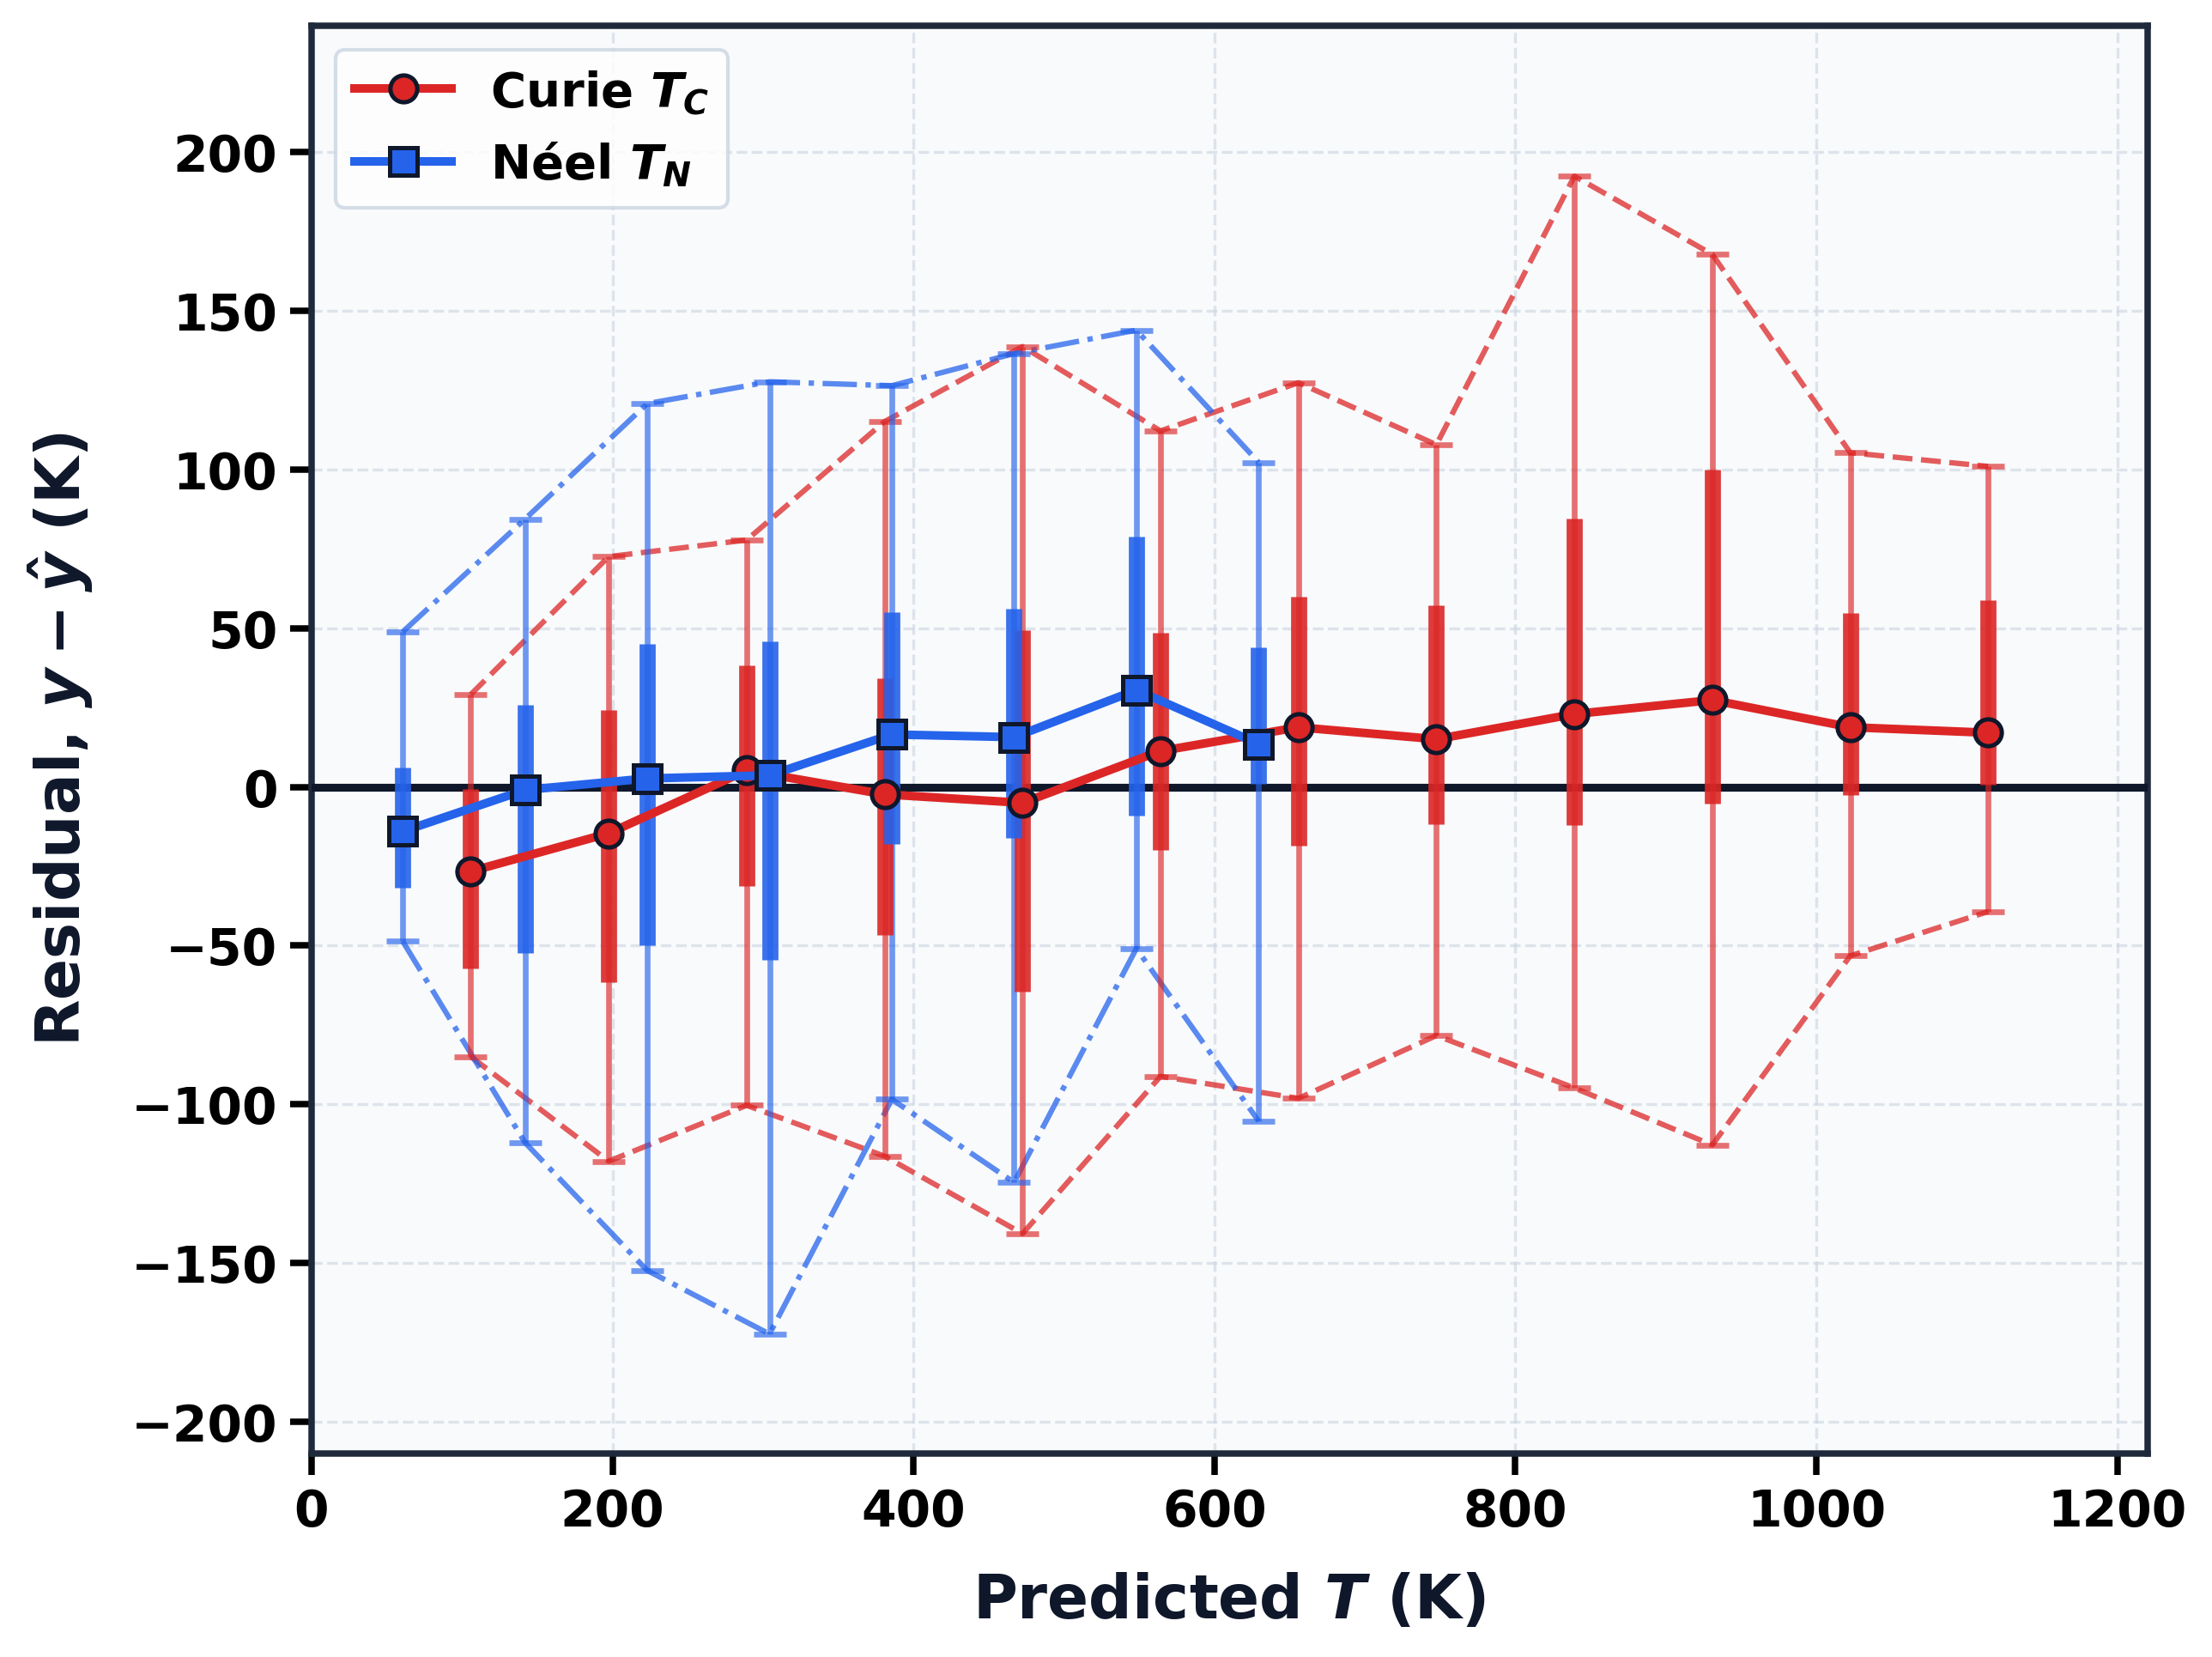
\includegraphics[width=\textwidth]{figures/residual_heteroscedasticity.png}
        \caption{Residual Distributions across Temperature}
        \label{fig:residual_plot}
    \end{subfigure}
    \caption{Uncertainty calibration and residual diagnostics. (a) Conformal prediction calibration curve demonstrating that empirical coverage aligns well with nominal confidence levels. (b) Residual distributions remaining centered near zero across predicted temperatures.}
    \label{fig:pair_conformal_residuals}
\end{figure}

\textbf{Candidate Screening:} The Pareto frontier (Figure~\ref{fig:pair_pareto_distributions}(a)) identifies candidates balancing $(BH)_{\max}$ and $T_C$. Crystal system distributions (Figure~\ref{fig:pair_pareto_distributions}(b)) confirm that tetragonal and hexagonal systems provide the highest share of high-$T_C$, high-anisotropy materials.

\begin{figure}[!t]
    \centering
    \begin{subfigure}[b]{0.485\textwidth}
        \centering
        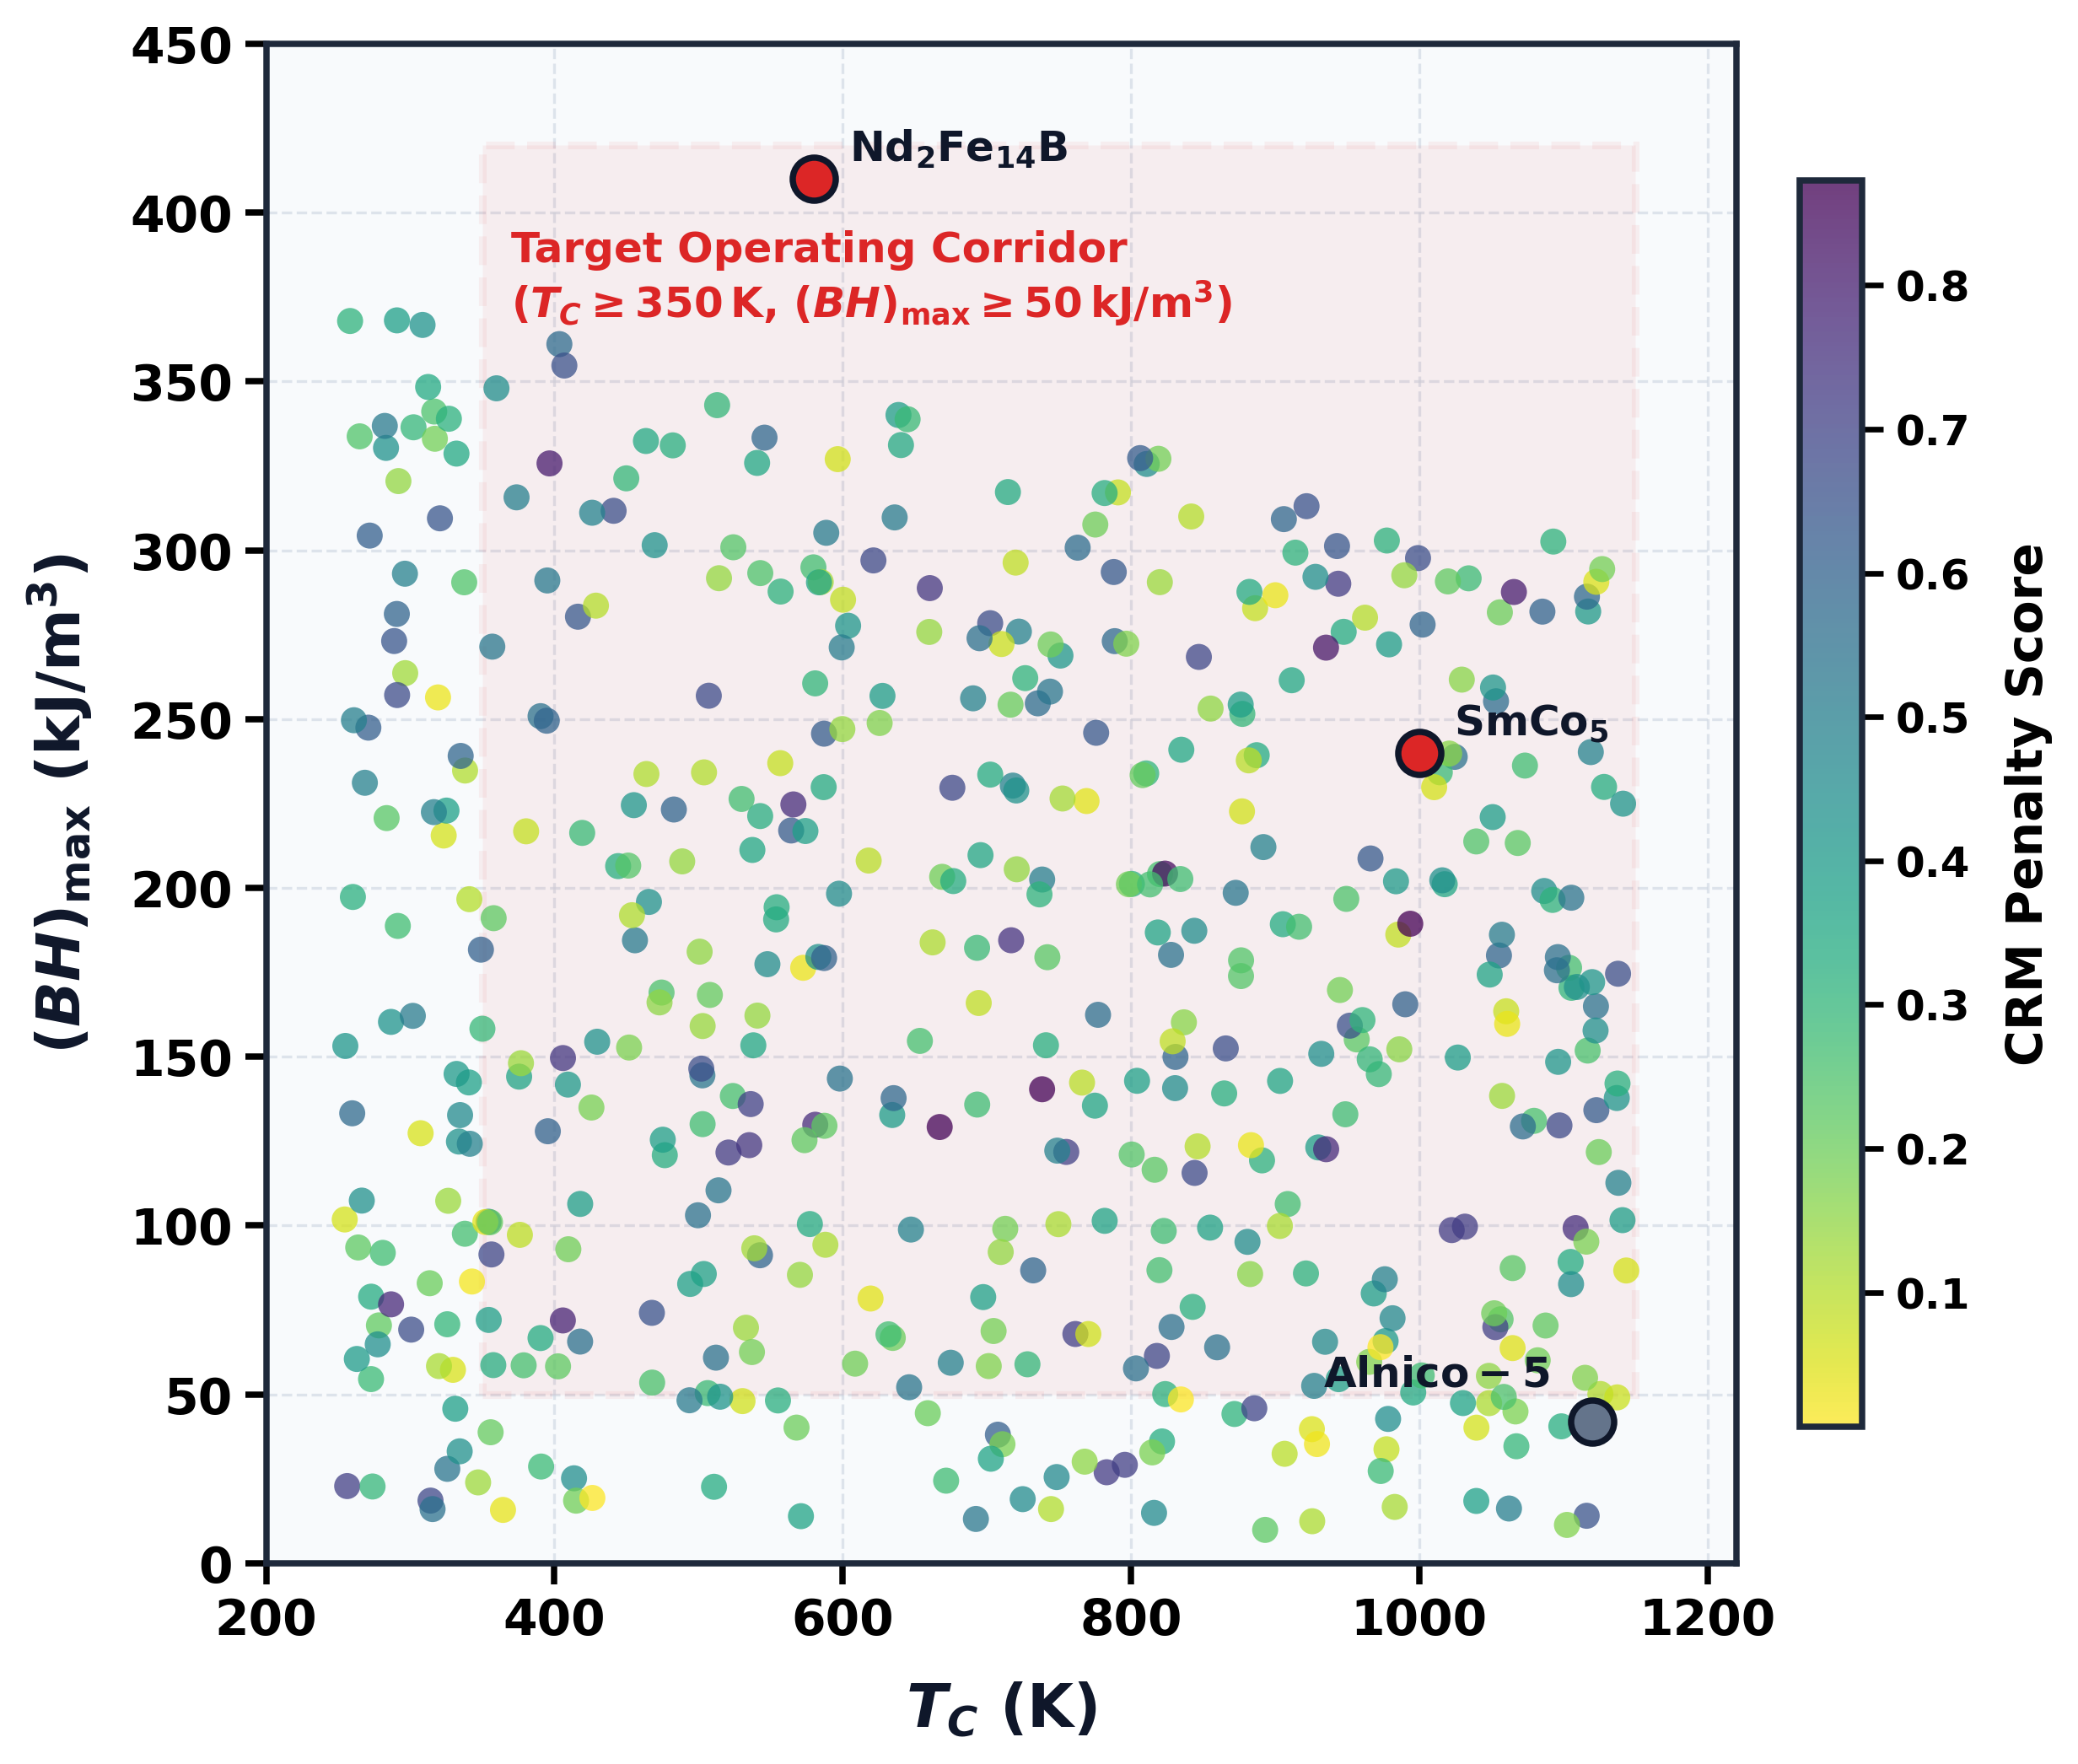
\includegraphics[width=\textwidth]{figures/discovery_pareto_frontier.png}
        \caption{Pareto Frontier ($(BH)_{\max}$ vs $T_C$)}
        \label{fig:pareto_frontier}
    \end{subfigure}
    \hfill
    \begin{subfigure}[b]{0.485\textwidth}
        \centering
        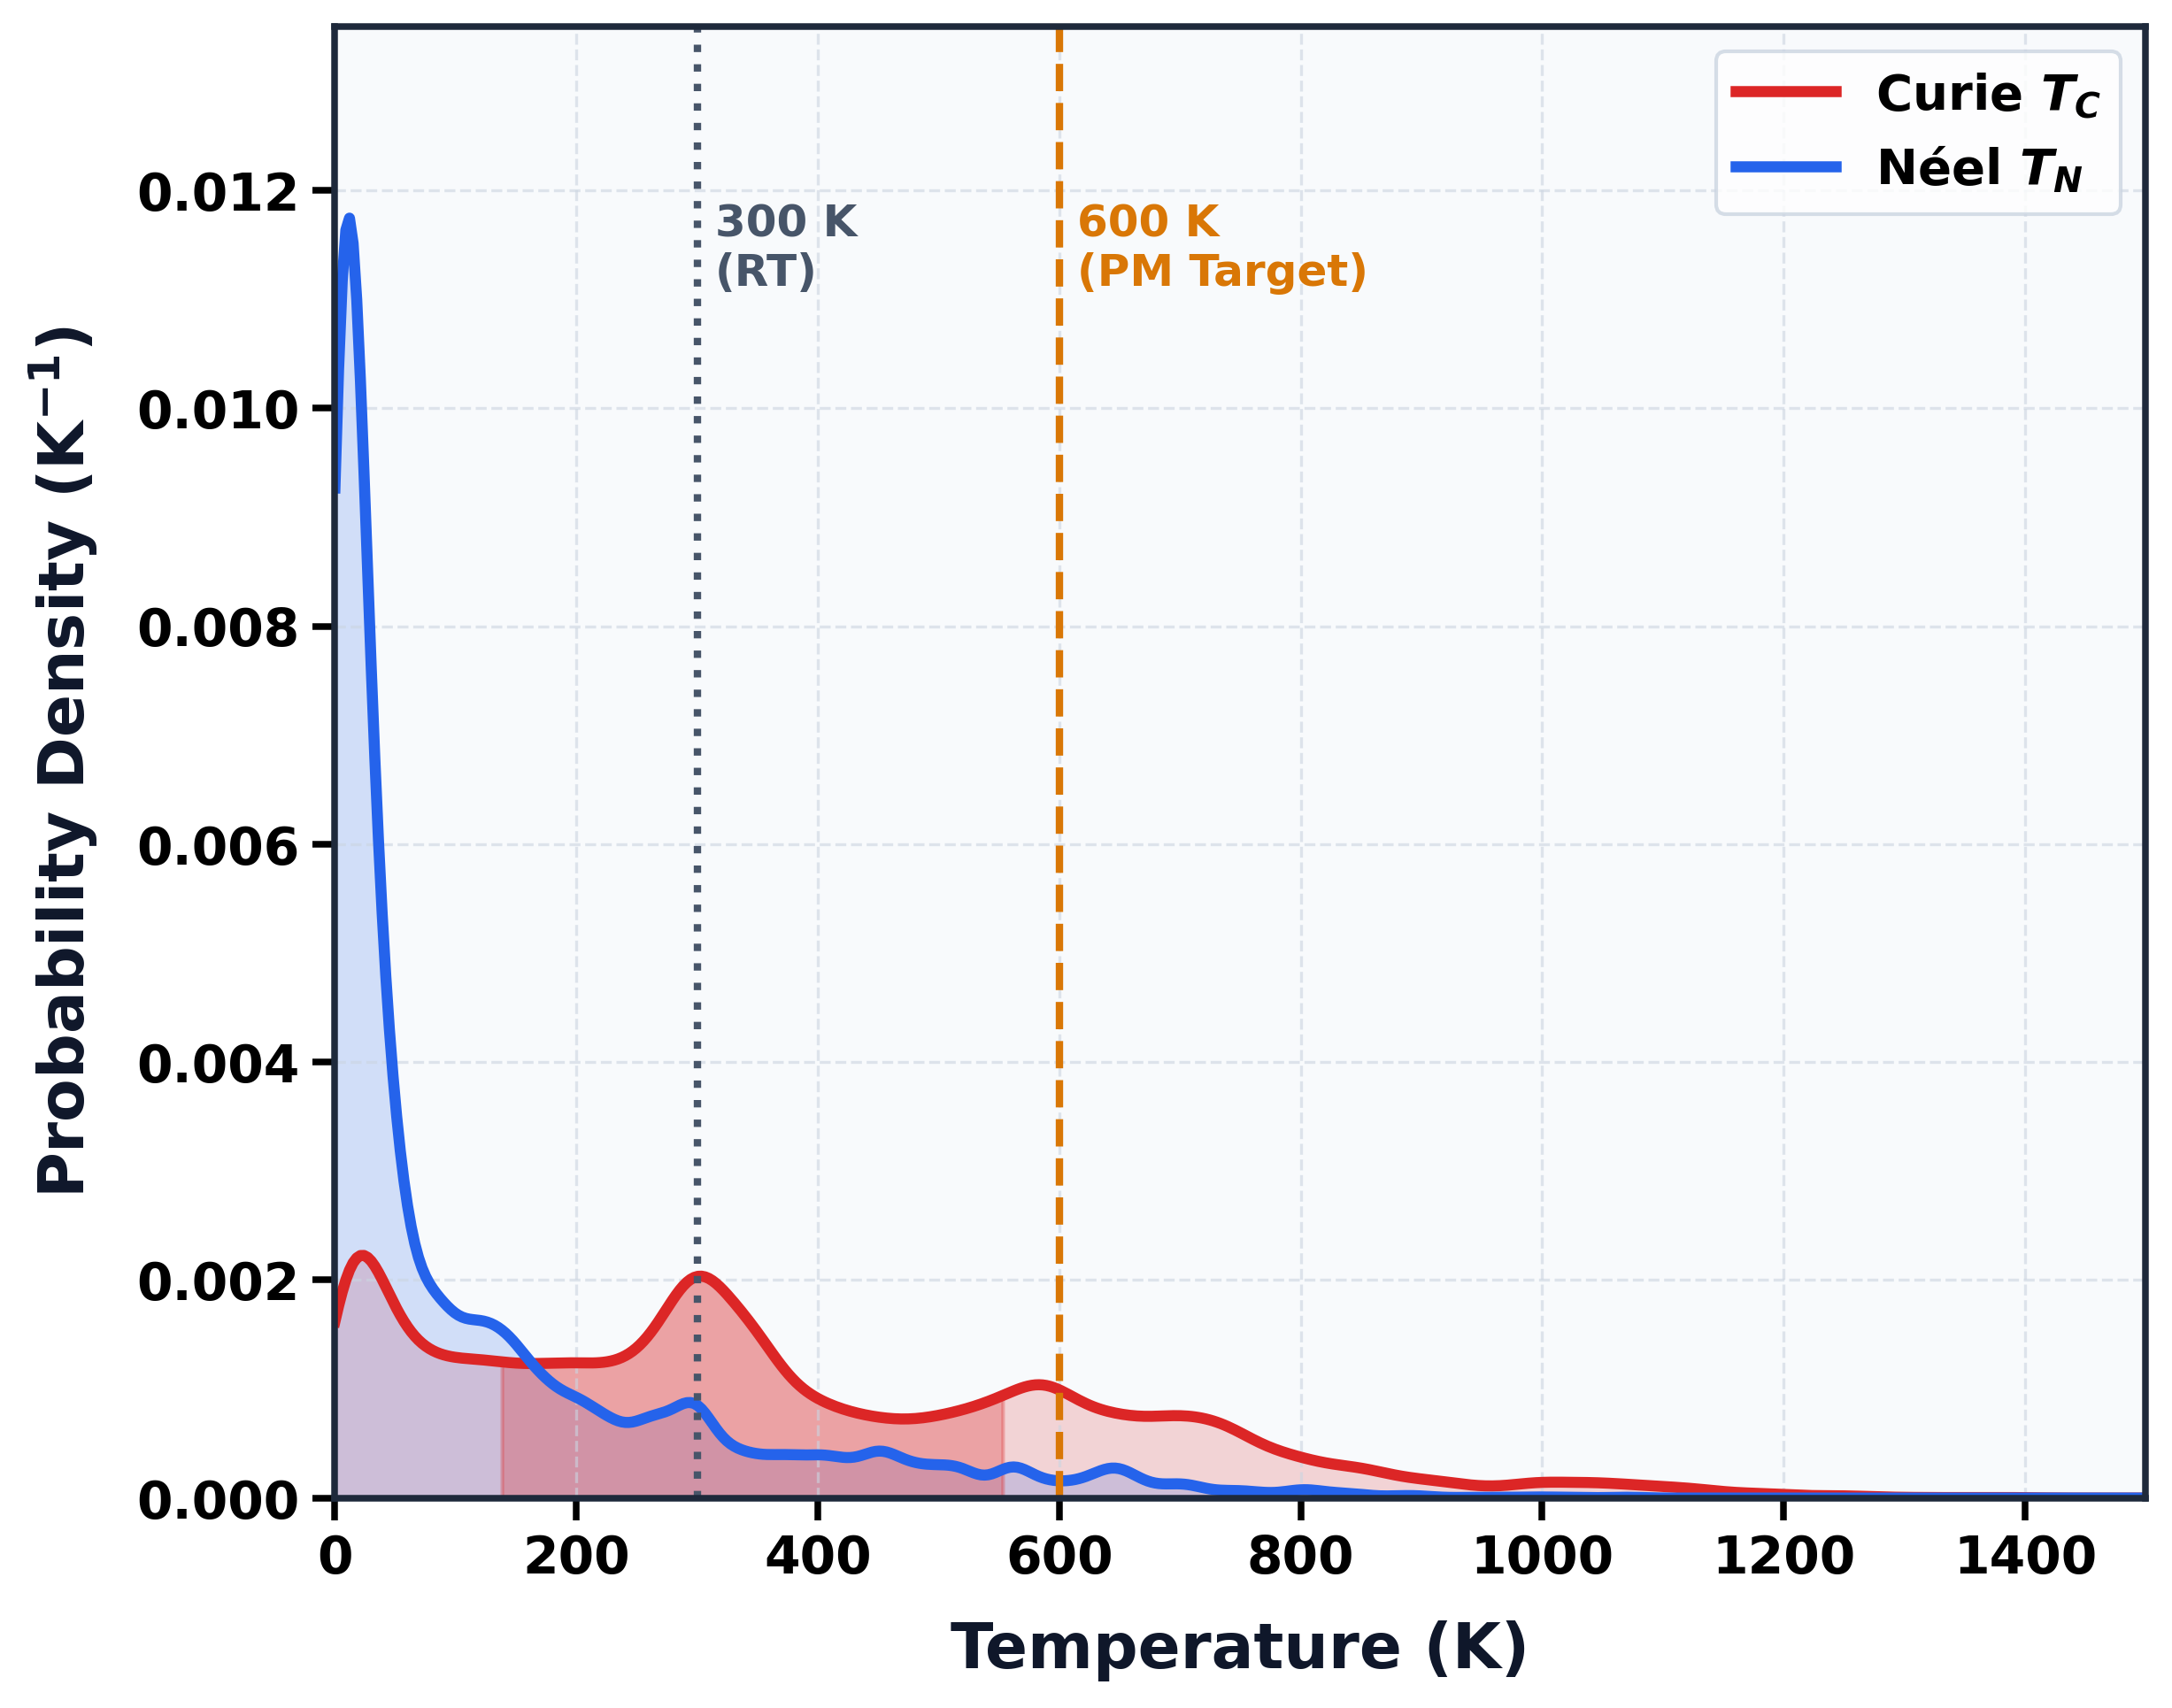
\includegraphics[width=\textwidth]{figures/transition_temperature_distributions.png}
        \caption{Transition Temperatures by Crystal System}
        \label{fig:temperature_distributions}
    \end{subfigure}
    \caption{Candidate screening and symmetry profiles. (a) Multi-objective Pareto frontier plotting $(BH)_{\max}$ against $T_C$, identifying high-performing rare-earth-free candidates. (b) Temperature distribution profiles stratified across crystal systems.}
    \label{fig:pair_pareto_distributions}
\end{figure}

% ==============================================================================
% 4. INTERACTIVE PLATFORM
% ==============================================================================
\clearpage
\section{Interactive Platform}

The MagMat-Discovery web application provides an interactive interface for candidate evaluation and screening (Figure~\ref{fig:streamlit_interface}), organized into four primary modules:

\begin{figure}[!t]
    \centering
    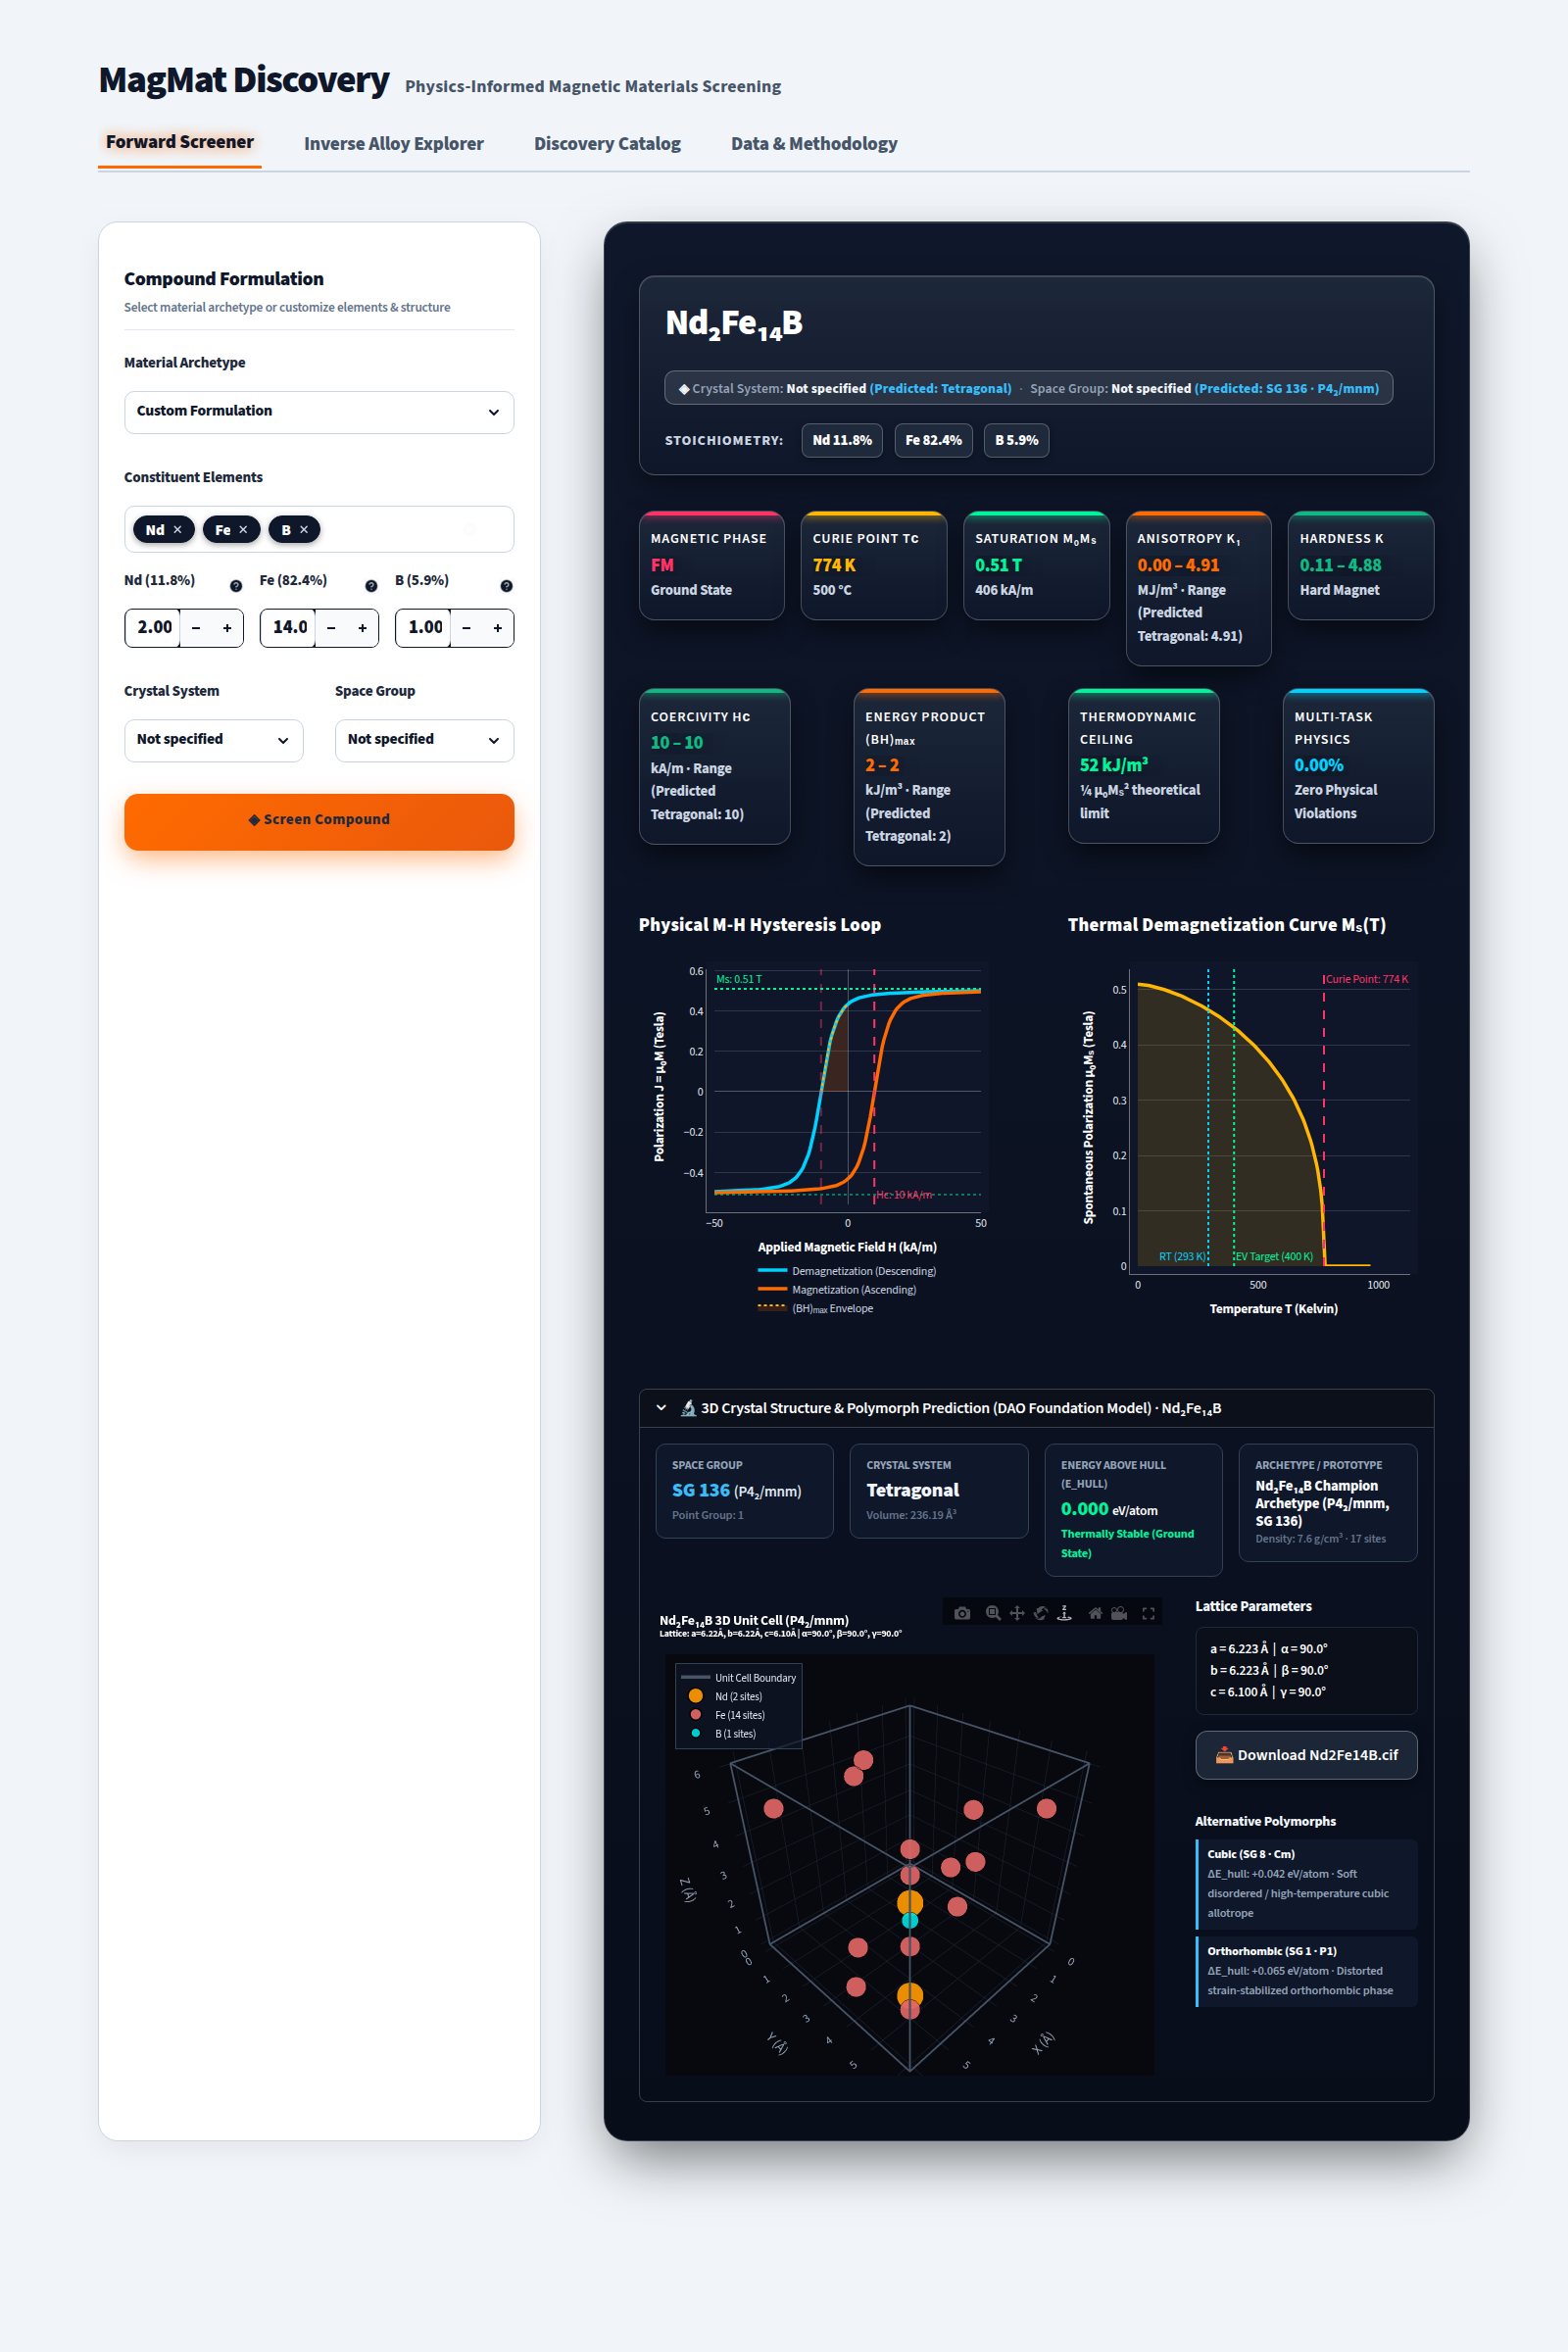
\includegraphics[width=0.62\textwidth,height=0.48\textheight,keepaspectratio]{figures/streamlit_app_interface.png}
    \caption{MagMat-Discovery interactive web platform interface. The forward screening dashboard displays predicted magnetic properties, multi-task physical consistency checks, simulated $M$-$H$ hysteresis loop, thermal demagnetization curve $M_s(T)$, and interactive 3D crystal structure for $\text{Nd}_2\text{Fe}_{14}\text{B}$.}
    \label{fig:streamlit_interface}
\end{figure}

\begin{itemize}[leftmargin=1.5em, itemsep=2pt]
    \item \textbf{Forward Screener:} Users enter a formula or select reference magnets ($\text{Nd}_2\text{Fe}_{14}\text{B}$, $\text{SmCo}_5$, Alnico, $\text{Fe}_{16}\text{N}_2$) to view property predictions with 90\% intervals, simulated $M$-$H$ loops, $M_s(T)$ curves, and 3D crystal structures.
    \item \textbf{Inverse Explorer:} Users set targets (e.g., $T_C \ge 500\,\text{K}$, $(BH)_{\max} \ge 120\,\text{kJ/m}^3$) and filter by composition, such as excluding critical rare earths (Nd, Dy, Sm).
    \item \textbf{Discovery Catalog:} Browsing and export of material records, with filtering along the Pareto efficiency frontier.
    \item \textbf{Reference Tab:} Dataset statistics, space group distributions, and validation metrics displayed in the app.
\end{itemize}

% ==============================================================================
% 5. SUMMARY AND OUTLOOK
% ==============================================================================
\section{Summary and Outlook}

MagMat-Discovery combines physical principles, graph neural networks, and micromagnetic rules to screen permanent magnets:
\begin{itemize}[leftmargin=1.5em, itemsep=2pt]
    \item \textbf{Accurate Screening:} Magnetic phase classification (91.9\% accuracy) and ordering temperatures ($R^2 = 0.82$ for $T_C$) serve as reliable initial filters.
    \item \textbf{Physical Ranking:} Extrinsic properties ($H_c, K_1, (BH)_{\max}$) achieve $R^2 = 0.46$--$0.62$, providing a grounded pre-filter to prioritize candidates for synthesis.
\end{itemize}

Future work will incorporate grain-boundary phase models, domain wall pinning, and integration with automated synthesis platforms.

% ==============================================================================
% REFERENCES
% ==============================================================================
\vspace{0.4cm}
{\small
\begin{thebibliography}{9}
\bibitem{nemad2025}
NEMAD Consortium, \emph{A non-equilibrium magnetic materials database and machine learning framework for magnetic materials discovery}, Nature Communications, \textbf{16}, 2025, doi:10.1038/s41467-024-55500-7.

\bibitem{materials_project}
A. Jain et al., \emph{Commentary: The Materials Project: A materials genome approach to accelerating materials innovation}, APL Materials, \textbf{1}(1), 011002, 2013.

\bibitem{mace2022}
I. Batatia, D.~P. Kovacs, G. Simm, C. Ortner, and G. Csanyi, \emph{MACE: Higher order equivariant and message passing neural networks for materials}, Advances in Neural Information Processing Systems (NeurIPS), \textbf{35}, 11423--11436, 2022.

\bibitem{dao2026}
Z. Huang et al., \emph{Siamese Foundation Models for Crystal Structure Prediction}, Nature Communications, \textbf{17}, 2026, doi:10.1038/s41467-026-72362-3.

\bibitem{kronmuller2003}
H. Kronmüller and M. Fähnle, \emph{Micromagnetism and the Microstructure of High-Technology Materials}, Cambridge University Press, 2003.

\bibitem{vovk2005}
V. Vovk, A. Gammerman, and G. Shafer, \emph{Algorithmic Learning in a Random World}, Springer, 2005.

\bibitem{coey2010}
J.~M.~D. Coey, \emph{Magnetism and Magnetic Materials}, Cambridge University Press, 2010.
\end{thebibliography}
}

% ==============================================================================
% APPENDICES
% ==============================================================================
\newpage
\appendix

\section{Physical Feature Formulations}
\label{sec:appendix_physics}

This appendix provides the formal equations for the physics-guided descriptors described in Section~\ref{sec:physics_descriptors}.

\subsection{Goodenough-Kanamori Superexchange}
In transition metal oxides, sulfides, and pnictides, indirect exchange between magnetic cations ($M$) mediated by non-magnetic anions ($X$) follows Goodenough-Kanamori rules. The transfer factor models the competition between ferromagnetic direct exchange and antiferromagnetic superexchange:
\begin{equation}
    J_{\text{ex}} \propto \cos^2\theta \cdot \exp\left( - \frac{|\chi_{\text{cat}} - \chi_{\text{anion}}|}{\chi_0} \right)
\end{equation}
where $\theta$ is the $M\text{--}X\text{--}M$ bond angle, $\chi_{\text{cat}}$ and $\chi_{\text{anion}}$ denote Pauling electronegativities, and $\chi_0$ is a characteristic scaling parameter ($\chi_0 \approx 1.5$). When $\theta \approx 180^\circ$, strong antiferromagnetic superexchange dominates; near $90^\circ$, ferromagnetic direct exchange is favored.

\subsection{Dzyaloshinskii-Moriya Interaction (DMI) Proxy}
In non-centrosymmetric space groups containing elements with strong spin-orbit coupling, the broken inversion symmetry introduces an antisymmetric exchange interaction (DMI) that induces chiral spin canting:
\begin{equation}
    D_{\text{proxy}} = \mathbb{I}(\text{non-centrosymmetric}) \sum_{i} x_i \left( \frac{Z_i}{100} \right)^4 \cdot \mathbb{I}(Z_i \ge 40)
\end{equation}
where $\mathbb{I}(\cdot)$ is an indicator function (equal to 1 if the condition holds, 0 otherwise), $x_i$ is the atomic fraction of element $i$, and $Z_i$ is its atomic number. The fourth-power dependence reflects the relativistic scaling of spin-orbit coupling ($\lambda_{\text{SOC}} \propto Z^4$).

\subsection{Crystal Field and Stevens Operator Hamiltonian}
In uniaxial crystallographic systems (tetragonal, hexagonal, and trigonal), the first-order magnetocrystalline anisotropy constant $K_1$ arises primarily from single-ion crystal field interactions:
\begin{equation}
    \mathcal{H}_{\text{CF}} = B_2^0 O_2^0 + B_4^0 O_4^0
\end{equation}
where $B_n^m$ are crystal-field parameters and $O_n^m$ are Stevens operator equivalents. The second-order operator is defined by:
\begin{equation}
    O_2^0 = 3 J_z^2 - J(J+1)
\end{equation}
where $J$ is the total angular momentum quantum number. The sign of the second-order Stevens factor $\alpha_J$ dictates whether the single-ion interaction favors an easy axis ($\alpha_J < 0$, uniaxial anisotropy $K_1 > 0$) or an easy plane ($\alpha_J > 0$).

\clearpage
\section{MagFormer Architecture Details}
\label{sec:appendix_magformer}

This appendix provides the network equations for the MagFormer composition graph transformer described in Section~\ref{sec:magformer_architecture}.

\subsection{Node Initialization and Projection}
Each constituent element $i$ in a chemical formula is embedded through a combination of discrete atomic number embeddings and normalized elemental physical features:
\begin{equation}
    \mathbf{h}_i^{(0)} = \mathbf{W}_{\text{node}} \left[ \mathbf{e}_{Z_i} \;\parallel\; x_i \;\parallel\; \mathbf{p}_i \right]
\end{equation}
where $\mathbf{e}_{Z_i} \in \mathbb{R}^{64}$ is a learned element embedding vector, $x_i \in (0, 1]$ is the atomic fraction, and $\mathbf{p}_i$ is a normalized vector of elemental physical properties (electronegativity, covalent radius, valence, and Stoner parameter).

\subsection{Pair-Bias Self-Attention}
Constituent elements interact via multi-head self-attention modulated by a learned pairwise relational bias matrix $\mathbf{B}_{ij}$:
\begin{equation}
    \mathbf{A}_{ij} = \text{softmax} \left( \frac{\mathbf{Q}_i \mathbf{K}_j^T}{\sqrt{d_k}} + \mathbf{B}_{ij} \right) \mathbf{V}_j
\end{equation}
where query ($\mathbf{Q}$), key ($\mathbf{K}$), and value ($\mathbf{V}$) projections are computed from $\mathbf{h}_i^{(l)}$. The pairwise bias $\mathbf{B}_{ij}$ is generated by passing elemental feature differences $|\mathbf{p}_i - \mathbf{p}_j|$ through a two-layer multi-layer perceptron.

\subsection{Leakage-Free Composition Pooling}
To aggregate the multi-element representations into a fixed-length composition vector without leaking task-specific targets, MagFormer uses a composite pooling operation combining fraction-weighted sums, masked maximums, and global means:
\begin{equation}
    \mathbf{z}_{\text{comp}} = \left[ \sum_{i=1}^N x_i \mathbf{h}_i^{(L)} \;\parallel\; \max_{i=1 \dots N} \mathbf{h}_i^{(L)} \;\parallel\; \frac{1}{N}\sum_{i=1}^N \mathbf{h}_i^{(L)} \right] \in \mathbb{R}^{384}
\end{equation}
where $L$ is the final transformer layer and $N$ is the number of elements in the formula. The resulting 384-dimensional representation encodes complex non-linear chemical interactions and is supplied as an input to the tabular ensemble models.

\end{document}
